%----------------------------------------------------------------
% FEUILLE DE STYLE ENSG au format Latex
% Création : sept. 2010 (D Lercier)
% Modifications sept. 2012 (T Coupin), aout 2015 (C Drouadaine)
%----------------------------------------------------------------

\documentclass{themeensg}
\usepackage[utf8]{inputenc}
\usepackage[T1]{fontenc}
\usepackage{lmodern} % load a font with all the characters
\usepackage{caption}
\usepackage{fancyhdr}
\usepackage{lastpage}
\usepackage[inline]{enumitem} % horizontal enumerations
\usepackage{tikz-uml} % UML
\usepackage{color} % pseudo code
\usepackage[procnames]{listings}
\usepackage{listings} % source code
\usepackage{mathtools}
\usepackage{float} % figures positioning
\usepackage[bottom]{footmisc}
\usepackage{pdfpages}

\pagestyle{fancy}
\fancyhf{}
 
\rfoot{Page \thepage \hspace{1pt} of \pageref{LastPage}}

%---Texte en filigranne---
\SetWatermarkText{}
%pour l'enlever : \SetWatermarkText{}
%-------------------------

%---Mes packages à moi---
\usepackage[english, frenchb]{babel}
%------------------------

%---Mes raccourcis---
\newcommand{\transpose}[1]{{}^t \! #1}
\newcommand{\ensg}{\textsc{Ensg}}

%---Defining subsubsubsections
\setcounter{secnumdepth}{4}
\setcounter{tocdepth}{4}
\makeatletter
\newcounter {subsubsubsection}[subsubsection]
\renewcommand\thesubsubsubsection{\thesubsubsection .\@alph\c@subsubsubsection}
\newcommand\subsubsubsection{\@startsection{subsubsubsection}{4}{\z@}%
                                     {-3.25ex\@plus -1ex \@minus -.2ex}%
                                     {1.5ex \@plus .2ex}%
                                     {\normalfont\normalsize\bfseries}}
\renewcommand\paragraph{\@startsection{paragraph}{5}{\z@}%
                                    {3.25ex \@plus1ex \@minus.2ex}%
                                    {-1em}%
                                    {\normalfont\normalsize\bfseries}}
\renewcommand\subparagraph{\@startsection{subparagraph}{6}{\parindent}%
                                       {3.25ex \@plus1ex \@minus .2ex}%
                                       {-1em}%
                                      {\normalfont\normalsize\bfseries}}
\newcommand*\l@subsubsubsection{\@dottedtocline{4}{10.0em}{4.1em}}
\renewcommand*\l@paragraph{\@dottedtocline{5}{10em}{5em}}
\renewcommand*\l@subparagraph{\@dottedtocline{6}{12em}{6em}}
\newcommand*{\subsubsubsectionmark}[1]{}
\makeatother

\usepackage{hyperref}

\makeatletter
\def\toclevel@subsubsubsection{4}
\def\toclevel@paragraph{5}
\def\toclevel@subparagraph{6}
\makeatother

%--------------------

%---Paramètres du pdf---
\hypersetup{
       backref=true,                           % Permet d'ajouter des liens dans
       pagebackref=true,                       % les bibliographies
       hyperindex=true,                        % Ajoute des liens dans les index.
       colorlinks=true,  %Colorise les liens : true pour version numérique, false pour version d'impression
       breaklinks=true,                        % Permet le retour à la ligne dans les liens trop longs.
       urlcolor= blue,                         % Couleur des hyperliens.
       linkcolor= blue,                       % Couleur des liens internes.
       bookmarks=true,                         % Créé des signets pour Acrobat.
       %bookmarksopen=true,                    % Si les signets Acrobat sont créés,
                                               % les afficher complètement.
       pdftitle={Clément Drouadaine Internship Report},               % Titre du document.
                                               % Informations apparaissant dans
       pdfauthor={Clément Drouadaine},                      % dans les informations du document
       pdfsubject={Internship report}           % sous Acrobat.
    }

%-----------------------



%-------------------------------------------------------------

\setcounter{tocdepth}{4} %profondeur de la table des matières
\setcounter{secnumdepth}{4}

\title{Developing a graphical user interface for the real-time ionosphere scintillation monitor}

%
%-------------------------------------------------------------
% Début du document
%--------------------------------------------------------------
\newlength\longest
\begin{document}
%--------------------------------------------------------------
\begin{titlepage}
%Inclusion des labels des entreprises
%Pour un seul label (à gauche), mettre NULL pour les 3e et 4e argument
%\enterprise 
\begin{minipage}{.5\textwidth}
  
\includegraphics[width=.5\linewidth]{images/logos/ensg_logo.png}
\end{minipage}
\begin{minipage}{.5\textwidth}
  \centering
  
\includegraphics[width=.5\linewidth]{images/logos/kartverket_logo.png}
\end{minipage}

%Prevents LaTeX from messing with spacing before and after colons
\shorthandoff{:}

%Inclusion du titre
\maketitle{Internship report \\ Cycle: 3\up{rd} year of engineering, GTSI specialisation}
{Aurora_Borealis_Norway.jpg}

\infos{Clément Drouadaine}{September 2015}
\end{titlepage}


%---Page du jury---
%---Page du jury---
\newevenpage
\thispagestyle{plain}
\section*{Jury}
%Prevents LaTeX from messing with spacing before and after colons
\shorthandoff{:}

\vspace{0.5cm}

\textbf{President of jury:} \\

Pierre-Yves HARDOUIN

\vspace{0.5cm}

\textbf{Host Company:} \\

Kartverket

\vspace{0.5cm}

\textbf{Internship training supervisor:} \\ 

Oddgeir KRISTIANSEN \par
Emmanuel BARDIÈRE, ENSG \par
Vincent DE OLIVEIRA, ENSG

\vspace{0.5cm}

\textbf{Educational person in charge of the engineering course:} \\

Serge BOTTON, IGN/ENSG/DE/DPTS

\vspace{0.5cm}

\textbf{School's professional training counsellor:} \\

Patricia PARISI, IGN/ENSG/DE/DSHEI

\vspace{1cm}

\copyright \hspace{0.3cm} ENSG

\section*{Internship from 05/05/2015 to 25/09/2015}
\vspace{0.3cm}
\textbf{Web diffusion:} $\boxtimes$ Internet \hspace{0.2cm} $\boxtimes$ Intranet ENSG

\vspace{0.3cm}
\textbf{Document situation:} 

\vspace{0.2cm}
\par
Internship report presented in the end of the 3\up{rd} year of engineer cycle

\vspace{0.3cm}
\newcounter{x}
\setcounter{x}{\getpagerefnumber{LastPage}-\getpagerefnumber{beginappendices}+1}
\textbf{Number of pages:} \getpagerefnumber{LastPage} pages including \arabic{x} annexes

\vspace{0.3cm}
\textbf{Host system:} \LaTeX
\vspace{1cm}
%------------------


\clearpage

\thispagestyle{empty}
\null\vfill

\settowidth\longest{\huge\itshape It's still magic even if you know;}
\begin{center}
\parbox{\longest}{
  \raggedright{\huge\itshape
  It's still magic even if you know how it's done.\par\bigskip
  }
  \raggedleft\Large\underline{A Hat Full of Sky}\MakeUppercase{, Terry Pratchett}\par%
}
\end{center}
\vfill\vfill

\clearpage

%------------------------------------------------------------------------------
% Remerciements
\selectlanguage{english}
\newevenpage
\chapter*{Acknowledgements}

I would like to thank my internship supervisor in the Norwegian Mapping Authority (NMA), Rune Hanssen, for all the help and support he provided me all along the internship, and his availability whenever I needed him.\\

Thanks also to the whole of the geodesy department team for their welcome and especially Yngvild Linnea Andalsvik for her help, and Geir Arne Hjelle for the non work-related times we had.\\

Last but not least, I would like to give a big thanks to Zuheir Altamimi to whom I resorted once more to find me this internship. Like last year, I contacted him after unfruitful researches on my own, and he managed to find me an internship where I wanted, in the field I wanted, and within 24 hours. Once more, thank you very much.

%---Résumé (français)---
\selectlanguage{frenchb}
\begin{abstract}
\thispagestyle{empty}
	\vspace{1cm}

	Le Moniteur de Scintillation Ionosphérique en Temps Réel (RTIS) est un logiciel développé par l'Autorité  Norvégienne de Cartographie (NMA) pour mesurer et quantifier la scintillation ionosphérique, dont un des effets est de diminuer la qualité des observations GNSS. Il est déployé dans douze stations d'observation, répartis dans toute la Norvège et la Mer de Norvège. \\
	La but de ce stage était de concevoir et de développer une interface graphique ergonomique qui pourrait être utilisée par la NMA pour surveiller toutes les stations du réseau RTIS en temps réel et modifier ou remplacer leurs fichiers de configuration.
	\vspace{1.5cm}
	
	\textbf{Mots clés :} interface, web, surveillance.
\end{abstract}
%-----------------------


%---Résumé (anglais)---
\selectlanguage{english}
\begin{abstract}
\thispagestyle{empty}
	\vspace{1cm}
	
	The Real-Time Ionospheric Scintillation Monitor (RTIS) is a software developed by the Norwegian Mapping Authority (NMA) to measure and quantify the ionospheric scintillation, whose effects include lessening the quality of GNSS observations. It is deployed in twelve observation stations, spread all across Norway and the Norwegian Sea.\\
	The goal of this internship was to conceive and develop an ergonomic Graphical User Interface (GUI) that could be used in the NMA to monitor all the stations of the RTIS network in real-time and to edit or replace their configuration files.
	\vspace{1.5cm}
	
	\textbf{Key words:} interface, web, monitoring.
\end{abstract}
%----------------------



%---Table des matières, des figures et des tableaux---
\newevenpage
\tableofcontents

\newevenpage
\listoffigures

%----------------------------------------------------

\newevenpage
\chapter*{Glossary and useful acronyms}
\addcontentsline{toc}{chapter}{Glossary and useful acronyms}

\begin{acronym}
  \acro{CPU}{Central Processing Unit}
  \acro{DE}{Direction de l'Enseignement = Education Department}
  \acro{DPTS}{Département du Positionnement Terrestre et Spatial = Terrestrial \& Spatial Positioning Department}  
  \acro{DSHEI}{Département des Sciences Humaines, des relations Entreprises et des relations Internationales = Social Sciences, Industry relations and International relations Department}
  \acro{ENSG}{École Nationale des Sciences Géographiques = National School of Geographic Sciences}
  \acro{ERR}{ERRor messages}
  \acro{FIFO}{First In, First Out}
  \acro{FTP}{File Transfer Protocol}
  \acro{GPS}{Global Positioning System}
  \acro{GLONASS}{GLObal NAvigation Satellite System}
  \acro{GNSS}{Global Navigation Satellite System}
  \acro{GTSI}{Géomatique et Technologie des Systèmes d'Information = Geomatics and Technology of the Information Systems}
  \acro{GUI}{Graphical User Interface}
  \acro{IGN}{Institut Géographique National = National Geographical Institute}
  \acro{IP}{Internet Protocol}
  \acro{IPC}{Inter-Process Communication device}
  \acro{MON}{MONitoring table}
  \acro{NMA}{Norwegian Mapping Authority, the English name of Kartverket}
  \acro{OS}{Operating System}
  \acro{PHP}{PHP: Hypertext Preprocessor (recursive acronym)}
  \acro{PROC}{list of active PROCesses}
  \acro{RTIS}{Real-Time Ionosphere Scintillation}
  \acro{SATREF}{SATellittbasert REFeransesystem = Satellite-based Reference System}
  \acro{SSH}{Secure SHell}
  \acro{TCP}{Transmission Control Protocol}
  \acro{UDP}{User Datagram Protocol}
  \acro{UML}{Unified Modelling Language}
\end{acronym}


%---Introduction------------------------------------------------------------------
\newevenpage
\chapter*{Introduction}
  \addcontentsline{toc}{chapter}{Introduction}
  Due to the high latitude of Norway and of the norwegian islands, the country is subject to space phenomena, dont une des manifestations les plus fréquentes are aurora borealis. They are also responsible for irregularities in the electron distribution in the ionosphere, that can directly impact the quality of GNSS observations across the country.\\ The Real-Time Ionospheric Scintillation monitor software has been developed to measure and quantify this phenomenon, and has been deployed in 12 stations all across the Norwegian Sea. These stations send their data to a server in Hønefoss, where the Norwegian Mapping Authority is located. This internship, however, has nothing to do with this data: it aims to see the creation of a new graphical user interface that would allow to easily monitor the stations of the RTIS network.
  \vspace{1.5cm}
	
%-------------------------------------------------------------------------------

\evenchapter[Definition of the objectives]{Definition of the objectives}

%-------------------------------------------------------------------------------
\section{What RTIS is: a brief overview}

\subsection{Space weather and scintillations}

The performance of GNSS systems can be severely affected by space weather. The main effects occur when the signals pass through the enhanced electron densities in the ionosphere. One of the main effects is a delay of the signal. This can to a certain degree be mitigated by using dual frequency. During high solar activity, the the electron density can be highly variable and the irregularities formed generate rapid fluctuations in the amplitude and phase of signals: this is also known as scintillations. The signal is scattered in random directions while propagating through the ionosphere causing it to interfere with itself. Amplitude scintillation may cause deep signal fades that can interfere with a user’s ability to receive GNSS signals. Phase scintillations can lead to increased phase noise, cycle slips, and even loss of lock if the phase fluctuations are too rapid for the receiver to track.\

\begin{figure}[hb]
	\centering
	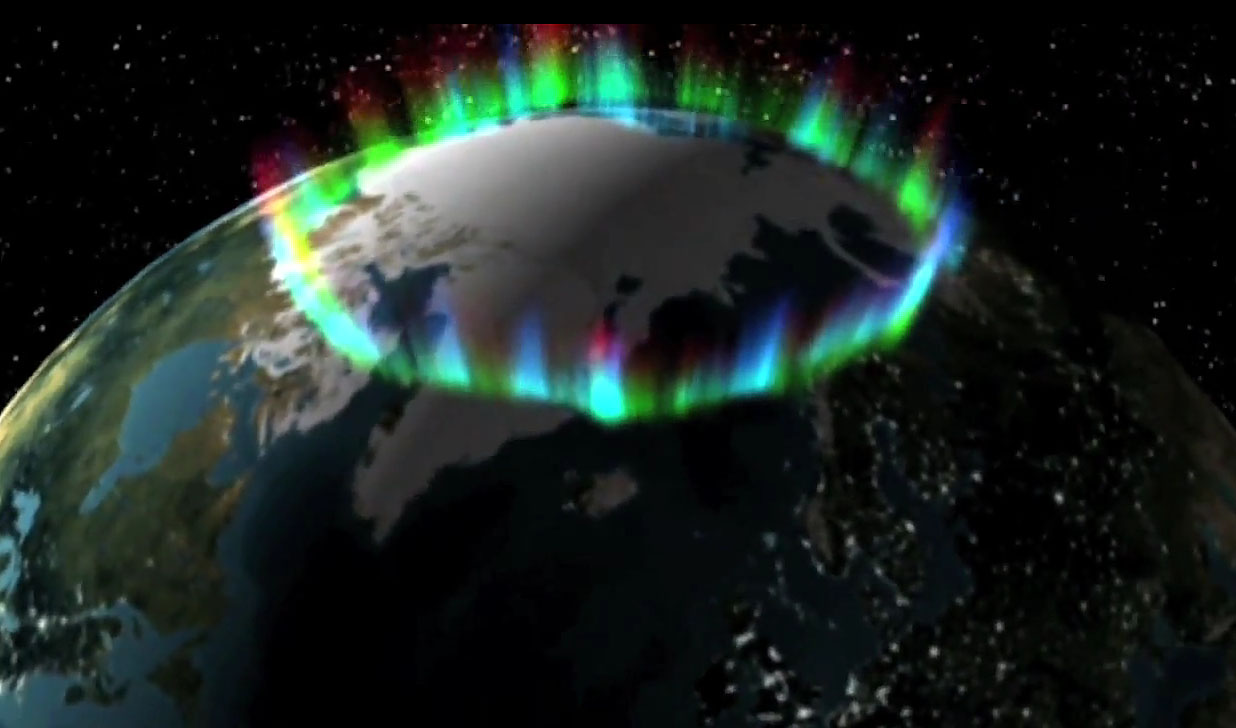
\includegraphics[width=0.7\textwidth]{auroral_oval}
	\caption{Auroral oval (Credit: NASA)}
\end{figure}

Equatorial latitudes and high latitude-regions are most severely affected by scintillations. Amplitude scintillations occur most commonly at equatorial latitudes, in particular the regions 15 degrees north and south of equator, while phase scintillations are more common at high latitudes. At high latitudes, scintillations are associated with processes in the polar cap and auroral oval. While the low latitude scintillations have clear seasonal and daily variations, the high latitude scintillations are more directly dependent on solar storms and the ionospheric activity that follows them.\\

\begin{figure}[ht]
	\centering
	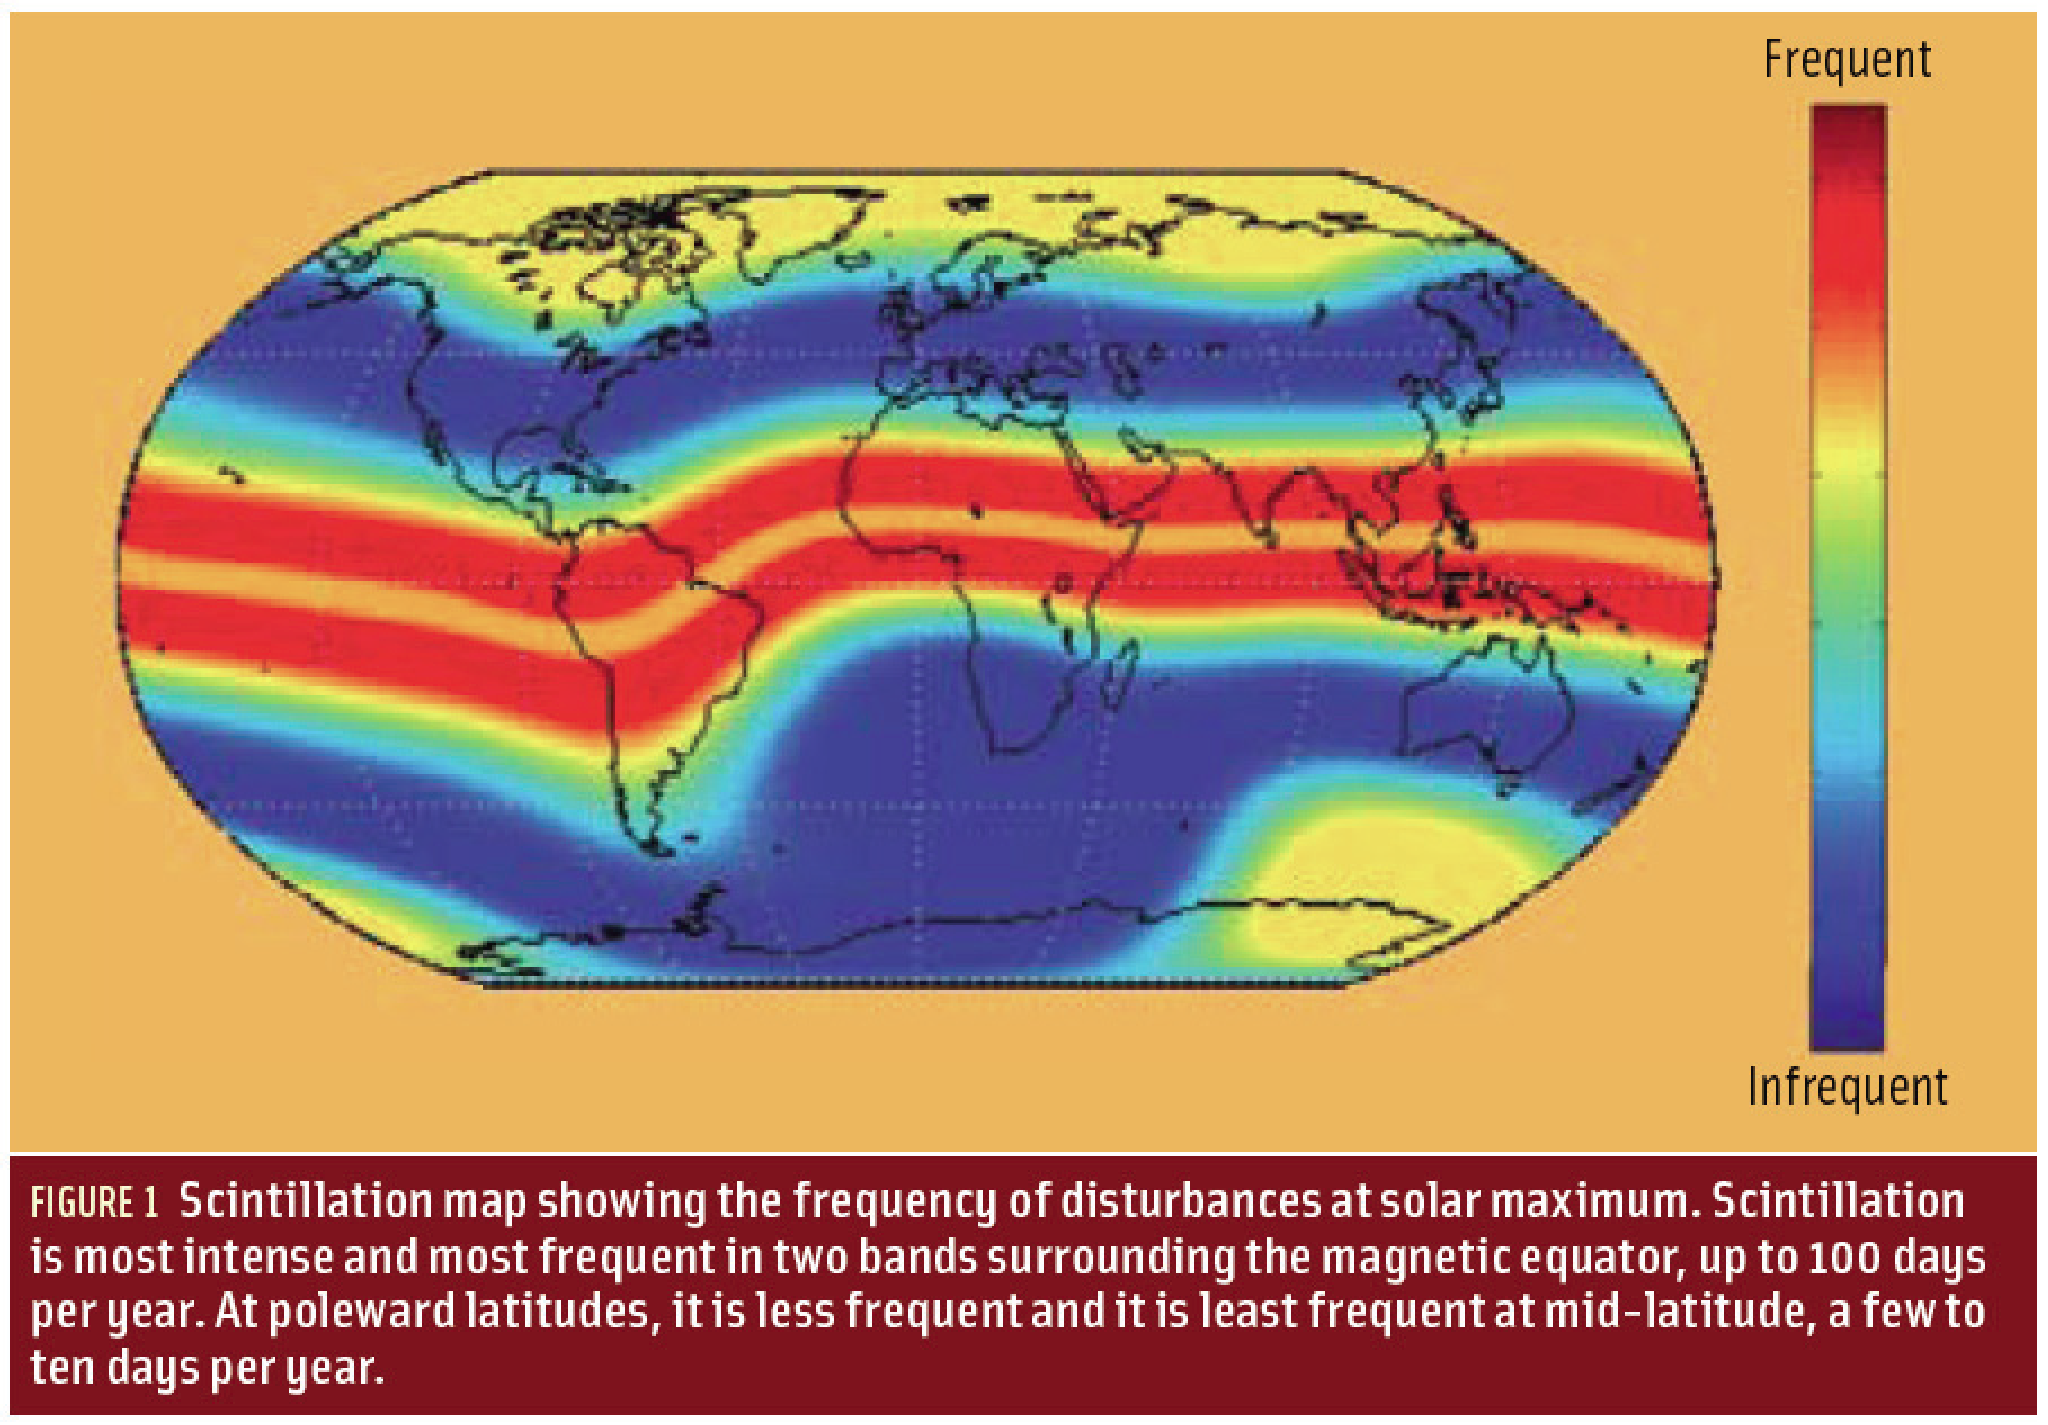
\includegraphics[width=\textwidth]{frequencyOfScintillation}
	\caption{Frequency of scintillations (P. Kintner, 2009)}
	\label{map}
\end{figure}

The scintillations are often quantified by the scintillation indices $\text{S}_{\text{4}}$ and $\sigma_\varphi$ for amplitude and phase scintillations respectively.

\subsection{RTIS receivers} 
The Real-Time Ionospheric Scintillation Monitor (RTIS) at the NMA is capable of detecting the occurrence of both amplitude and phase scintillation by providing numerical data and maps of the $\text{S}_{\text{4}}$ and $\sigma_\varphi$ indexes. Currently, the NMA operates 11 Septentrio PolaRxS scintillation receivers, deployed in Norway, in Iceland and in Faroe Islands. Additionally, one receiver is located at Hønefoss (NMA headquarters) for testing purposes. The receivers support multi-constellation and multi-frequency measurements, so that scintillation indexes are determined for both GPS and GLONASS data. Raw data measurements necessary for determining the scintillation indexes, such as signal phase, Doppler values, signal intensity and signal-to-noise ratio are carried out using a sampling rate of 100 Hz. \\
 
\begin{figure}[!hb]
	\centering
	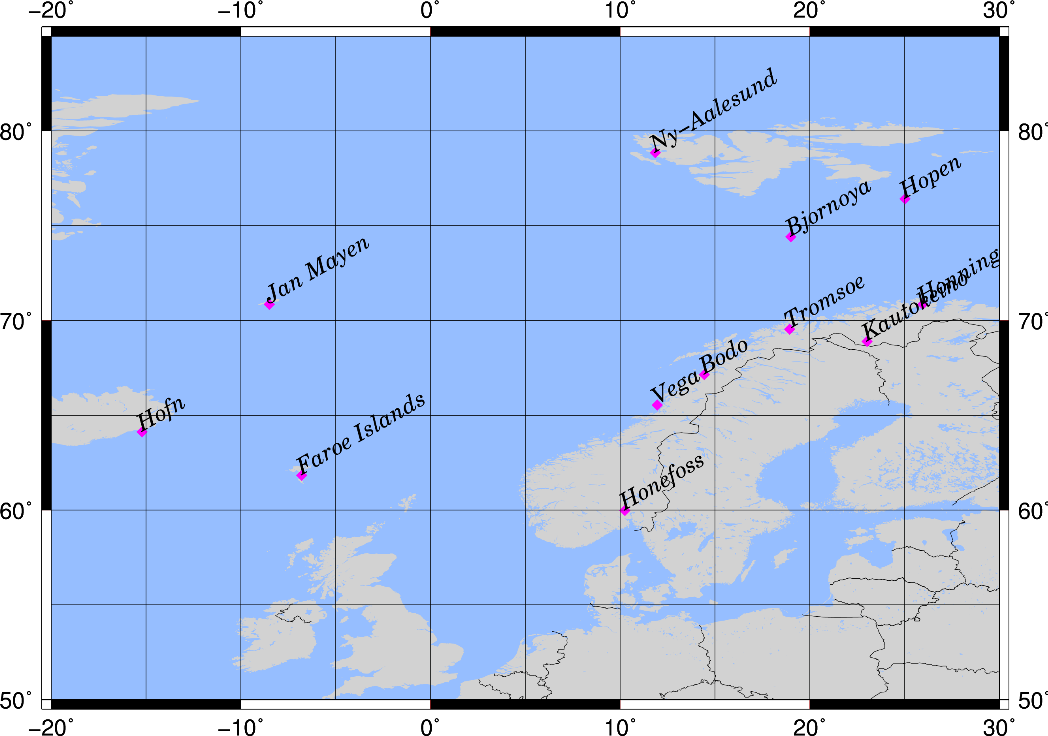
\includegraphics[width=0.9\textwidth]{rtisMap}
	\caption{Map of NMA scintillation receivers}
\end{figure}

\subsection{Operational environment}
The software is running on Lenovo PCs with Linux Lubuntu 32 bits environment. In addition, an external USB hard drive (of at least 2TB) is connected to the PC. The external hard drive is used for the raw data transport to NMA.\\

The RTIS software stores the raw data from the receiver and calculates the scintillation indices $\text{S}_{\text{4}}$ and $\sigma_\varphi$ in real time. 
The software tool performs the following main tasks:
\begin{itemize}
\item Calculate the scintillation indices $\text{S}_{\text{4}}$ and $\sigma_\varphi$ indices in one minute resolution.
\item Produce a message with 1 Hz observation data and send it to Hønefoss.
\item Produce raw data files necessary for the determination of scintillation parameters.
\item Produce output files containing the scintillation indices. 
\item Produce and send messages containing the scintillation indices and send them to the control centre in Hønefoss.
\end{itemize}

\clearpage
%-------------------------------------------------------------------------------

\section{What exists to monitor it: description of the existing}

As we have seen, RTIS data transfers have been fully implemented, and do not need any further work. The current RTIS application contains an alarm server and a simple monitor function. The alarm server can be configured to output alarms and info messages to various devices such as the console, an error log file and/or a special internal interface, IPC, which can be used by external applications to retrieve alarm and information messages in real-time. This IPC is a ringbuffer based on the FIFO principle. 

The monitor function is based on another IPC, which consists of a couple of tables that is accessible for external applications as shared memory. The table values are not real-time values, but are updated at various intervals.

To monitor the RTIS application, the alarm server is currently configured to print alarm messages to the console (of the remote station) and to files. By connecting to the console window, or downloading the alarm log files, status information and alarms can be retrieved both in real-time and as historical data.

To view the content in the monitor table, a console program called rtis\_mon, has been developed, which has to be started in a separate window.

\begin{figure}[ht]
	\centering
	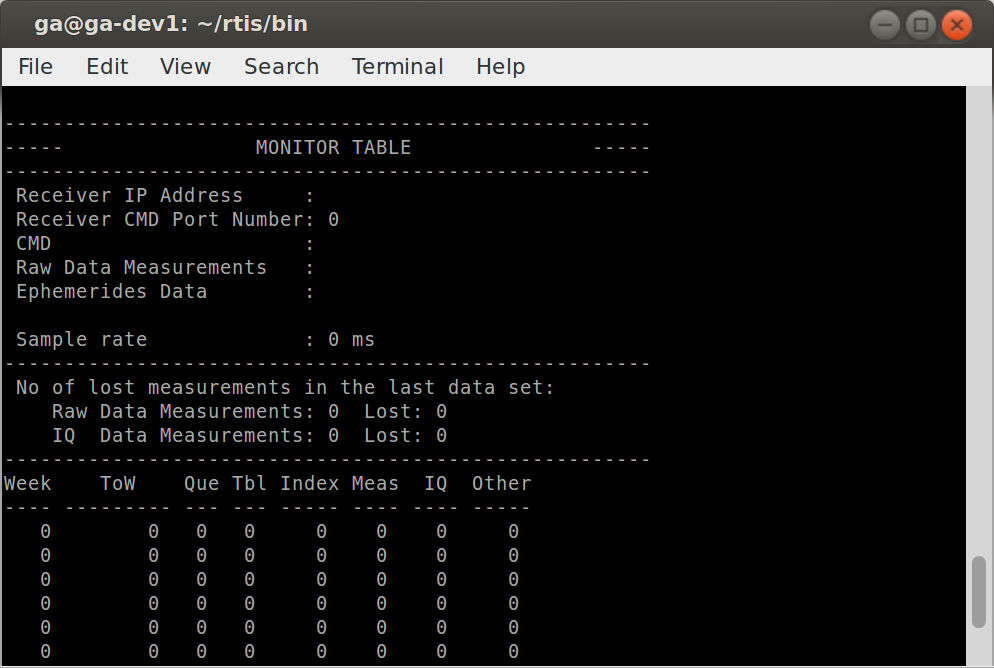
\includegraphics[width=0.8\textwidth]{rtis_mon}
	\caption{Monitoring table as seen with rtis\_mon}
\end{figure}

Although this method works, a few problems arise.
\begin{itemize}
	\item The process of connecting to the distant RTIS station via SSH is not intuitive, and requires the user to have a list of the IP addresses of all the remote stations, to look through it to find the one he wants, and then to enter the command in a terminal. This does not allow to quickly browse through all stations or to easily switch between two of them.
	\item To modify the configuration file, the editing can be made locally and transferred by FTP to the remote site or remotely, using an editor on the remote computer. While manageable, this method is not optimal.
	\item The update frequency cannot be chosen by the user. Though it is not a big issue, it can be annoying for the list of active processes for example, which is not going to change a lot, and certainly not every second.
\end{itemize}

%-------------------------------------------------------------------------------

\section{What needs to be done: goals and expected functionalities}

The making of a new Graphical User Interface (GUI) obviously aims at solving the aforementioned problems. Most of the requirements have been stated in my Statement of Work, in Annexe~\ref{SOW}. They will be detailed here. \\


The GUI should be a web application, preferably a light client that requires no installation whatsoever on the user side. The new GUI should allow the user to quickly see the status of every station, to connect to any of them, and to see any of the monitoring table, the list of active processes on the remote station, or the error messages\footnote{The \textit{error message} denomination encompasses all of the status messages returned by the applications within the RTIS system. The denomination can be misleading, since this also includes success messages.} returned by the software, to reboot the whole RTIS software, or to change its configuration file It combines both the status information obtained from the alarm system and the monitor data. 

In the following, we will refer to the monitoring table as MON, the list of active processes as PROC, and the error messages as ERR.\\

\subsection{Visualising data}

It should be possible to see any combination of MON, PROC and ERR simultaneously, and to have independent user-defined refresh frequency on each of them\footnote{"The data stream (process info, monitor data, event messages, status info) shall have a configurable update rate."}. For example, one should be able to choose to see both MON, refreshed every 2 seconds, PROC, refreshed every 3 minutes, and no error message. The "real-time" factor is not very important, as the data will not be subject to high-frequency changes. A delay of a few seconds is acceptable.\\

Displaying ERR should work differently than for PROC and MON: there will be no refresh frequency for it, and messages will always be displayed as soon as they are sent by the RTIS software. It should be possible, however, to filter them by their severity. Indeed, each error message within the RTIS software has a severity level. Ranked by order of magnitude, the possible levels are: \begin{enumerate*}
  \item Fatal
  \item Error
  \item Warning
  \item Info.
\end{enumerate*}
There are also two special unranked levels, Debug and Notice. The user should be able to select a severity level between 0 and 4, and to receive all error messages with a severity lower or equal to the selected level. Choosing the level 2, corresponding to Error for example, should make visible every message with a severity of Error or Fatal. The user should additionally be able to choose whether he wants any of Debug or Notice messages, regardless of the "main" severity filter he chose.

\subsection{Modifying the RTIS behaviour}

The GUI should not only be able to observe what the RTIS software does, but also to act on it in some ways: it should be possible to change the RTIS configuration file, and to reboot the whole RTIS software.\\

There are no specification on how modifying the configuration file should be handled. However, a new feature to add is a history of the previous configuration files. It should be possible to retrieve a previous configuration file, and to revert back to it. It should be noted that a change in the configuration file will not take effect until the RTIS is rebooted. It is thus possible to edit the configuration file several times in a row without actually changing anything, just to store the configuration files in the history for later. Again, there is no specification on how the storage should be done.

\begin{figure}[ht]
	\begin{center}
		\begin{tikzpicture}
		\begin{umlsystem}[x=4, fill=red!10]{The Graphical User Interface}
		\umlusecase[y=0, width=2cm]{See state of every station}
		\umlusecase[y=-4, width=2cm]{Connect to a station}
		\umlusecase[x=4, y=-1, width=2cm]{Visualise data}
		\umlusecase[x=4, y=-3, width=2cm]{Load config file}
		\umlusecase[x=4, y=-5, width=2cm]{Send config file}
		\umlusecase[x=4, y=-7, width=2cm]{Reboot}
		\end{umlsystem}
		
		\umlactor[y=-2]{user}
		
		\umlassoc{user}{usecase-1}
		\umlassoc{user}{usecase-2}
		\umlextend{usecase-2}{usecase-3}
		\umlextend{usecase-2}{usecase-4}
		\umlextend{usecase-2}{usecase-5}
		\umlextend{usecase-2}{usecase-6}
		\end{tikzpicture}
	\end{center}
	\caption{Use-case diagram of the GUI}
\end{figure}

\subsection{The problem of the bandwidth}

The stations of the RTIS network are scattered around in Norway and in the Norwegian Sea. Most of these stations are located close to inhabited locations and benefit from good and reliable connections to the internet.\\

But some stations have been placed in extremely remote locations, like Bjørnøya\footnote{see Fig.~\ref{map}} (\textit{Bear Island} in Norwegian), whose entire internet traffic transits through satellite connections. Due to the costs of bandwidth using these communications, the available bandwidth is very low, and due to the island being more than 74\degre north, even the satellite connection is unreliable and can be subject to unpredictable interruptions. \\

Moreover, there is already data transiting through this connection: the actual observation data that is sent to the control centre. One of the requirements for the new RTIS GUI is thus to minimise the amount of data sent or received, to be sure that every message could be received on time, and would not conflict with the observation data for the bandwidth access. The number of exchanges and/or the size of messages exchanged between the GUI and the stations should be as small as possible.\\

It is also a requirement that the remote RTIS station should detect if the connection with the GUI had been broken, and would then stop sending data through a broken pipe. The user should still be able to cleanly disconnect from the station to stop receiving data from it, but in the event of a breakage of a connection, the station should also be able to detect it by itself and not indefinitely continue sending data while waiting for a disconnection signal from the GUI.

\subsection{Miscellaneous}
The website should be able to be visited on any kind of device, with any kind of OS: Linux and Windows computers, Android and iOS phones... This has technical implications and implies to check compatibility when choosing technologies, and also influence the design of the web page, which should be responsive and adapt to mobile devices with a smaller screen.\\

About the languages to code the website in, the choice is limited to PHP or Java. Although some other  technologies might be tempting, like Node.js for the real-time display, all the future maintenance of my work is going to be done by the team behind RTIS, and they logically chose to limit the technologies involved to ones they were familiar with.\\

It is not required to have any login system, nor to be able to deal with simultaneous users on the GUI. It is only meant for an internal use, with restricted access. Anyone able to access the website is able to do all the interface allows to do. I am not aware of the internal workings of the internal network in NMA, and am only expected to have the product working on my development server. They will deal with the deployment.

%-------------------------------------------------------------------------------
\evenchapter[The proposed solution]{The proposed solution}
%-------------------------------------------------------------------------------
\section{General considerations}

The solution I have come up with is a light client: since there are no calculations nor any resource-consuming operation that is going to be needed, everything will be done on the web server without any risk of overloading it.\\

The website is coded in PHP, because it is a language I and the RTIS team are familiar with. Moreover, while environments like J2EE could be useful for bigger projects, this relatively simple interface does not require such a complex technology.
As the RTIS program is written in C and includes some low level libraries for communications, all of the code behind the interface used to communicate with the RTIS system will be written in C as well.\\

Also, while the GUI can ask for the RTIS software to send data, it cannot directly retrieve it: some modules have to be added to interact with the RTIS software, in the distant stations, to be able to communicate with them.

\section{Architecture}
\subsection{Global overview}

\begin{figure}[!hb]
	\centering
	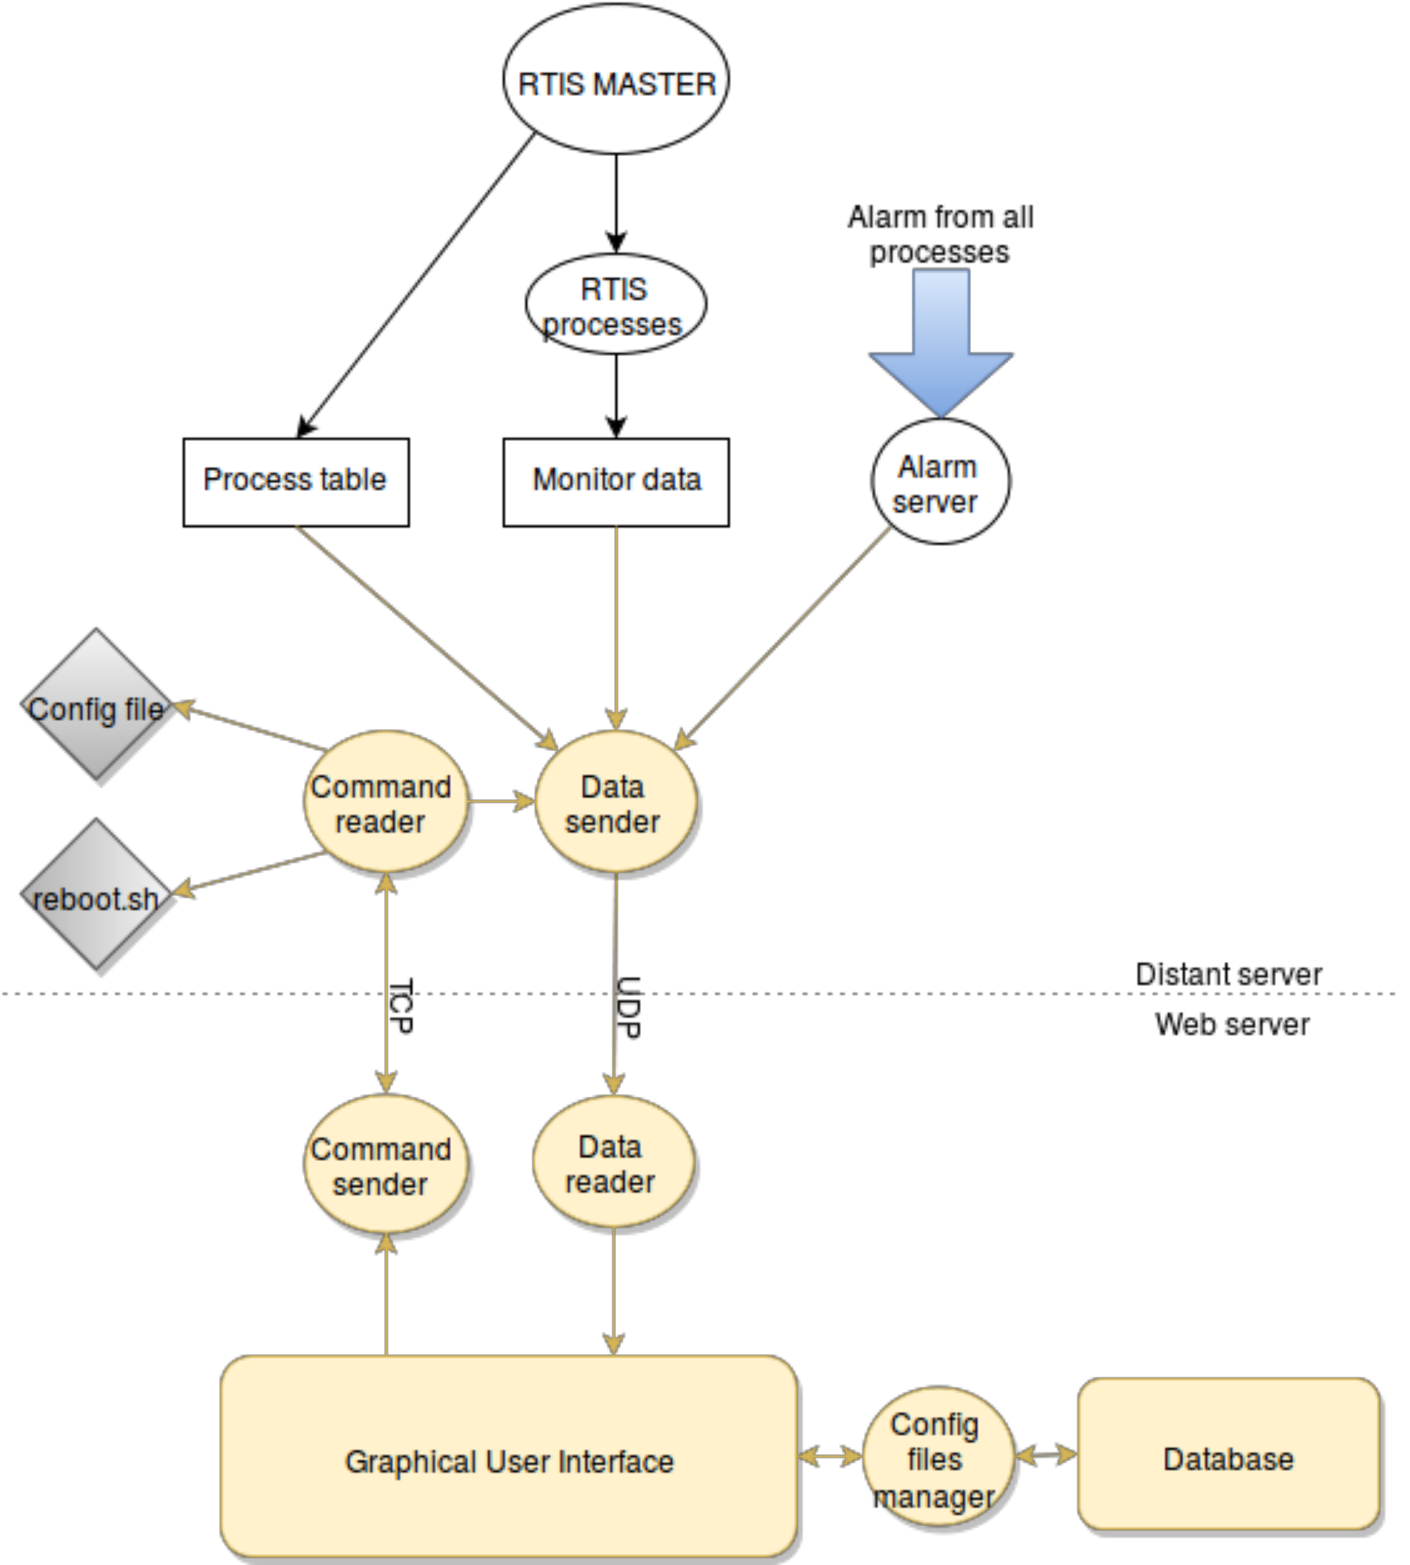
\includegraphics[width=0.8\textwidth]{global_flowchart}
	\caption{General organisation of the solution, working document}
	\label{generalOrganisation}
\end{figure}

The general architecture of my solution is presented in figure~\ref{generalOrganisation}.

In white, we have a schematization of the existing RTIS software, which will be described more in detail below, and in yellow are a simplified version of the modules and programs I have developed.

\subsubsection{A brief overview of the RTIS software}

First, let us go through the existing RTIS software to better understand how I will interact with it. Right on top, we have the GNSS receiver, whose role is obviously to collect data. This data is stored into one of the two data buffers, while the other one is being processed by the RTIS software. Every minute, the buffers are swapped. Every buffer contains one minute of observations, which implies that RTIS can take up to one minute to process one minute of data. If it takes longer, the swapping cannot occur and the RTIS software stops, and sends a fatal error. Hence the need for the modules I add to take as little resources as possible so that the processing software is able to perform its work within the one-minute time limit.\\

Just underneath the GNSS receiver, we have the Controller. It is responsible for managing all the modules that do the processing, ensuring that they are all up and running, and relaunching them if necessary. To reboot the whole RTIS system, one only needs to reboot the Controller.\\

The interface between the GUI and the RTIS software consists in the three aforementioned IPCs: the process table, the monitor data and the alarm ringbuffer. We do not need to know any more about the inner workings of the software or its data.

A description of the process table and the monitor data structures as returned by the IPCs is available in Annexe~\ref{structures}. The error messages simply consist of formatted strings.

\subsubsection{The general idea behind the architecture}

We will here refer to the web server that hosts the GUI as "the client" and to the distant RTIS installation as "the server".
The architecture is pretty straightforward: the GUI can send commands to the server via the \textit{Command Sender}, which are then read on the server by a dedicated \textit{Command Reader}. Depending on the message, the \textit{Command Sender} will either ask for data to be sent by the \textit{Data Sender}, update the configuration file on the server, or launch a bash script to reboot the system. The \textit{Data Sender} reads data from the RTIS IPCs according to what the \textit{Command Reader} demands, and sends it back to the GUI, which then reads and displays it.\\

There are two types of connections that link the server to the server: the client sends its request using the TCP protocol, while the server sends its data using UDP. The reason for that is that the TCP protocol offers a reliable connection: whenever a message is sent through a TCP stream, the receiver has to send a confirmation of the reception of the message, and if the sender does not receive the confirmation, it will send the message again up to 5 times before giving up. As we want to be sure that our commands have been sent, this is the solution to use here.
The UDP protocol, on the other hand, does not perform any check, nor needs the receiver to actually be connected. It just sends data and hopes that it will be received on the over side. Although obviously less reliable than TCP, it is also much faster for real-time applications: if the message has not been received, there is no point in trying to re-send it as it is already obsolete, and we need to send new messages with the new data instead. What matters here is sending information quickly, and if some of it is lost, it is not a major problem.\\

About the history of configuration files, now. To limit the use of bandwidth, whenever the user wants to view the history of the configuration files for a station, or even the current configuration file, it is not efficient to fetch it from the server: even though these files only weigh 2 kB, this would result in unneeded bandwidth usage.
A database has thus to be created on the client, where configuration files are duplicated whenever they are sent to the server. This way, we are ensured to always have all of the configuration files handy without any need for costly data transfer.


\subsection{In-depth descriptions of the modules}

\begin{figure}[!h]
	\centering
	\includegraphics[width=\textwidth]{detailed_flowchart2}
	\caption{Detailed organisation of the modules, working document}
\end{figure}

First of all, all communications between client and server are made via SATREF messages. Their specification is given in Annexe~\ref{satref}. It is an efficient and easy-to-implement way of communication.

\subsubsection{Command senders}

\begin{figure}[hb]
	\begin{tabular}{|c|c|c|}
	  \hline
	  Short name & Message type & Signification \\
	  \hline
	  CFG & 20 & Contains a new configuration file to replace the current one \\
	  PROC & 21 & Asks for the Process Table to be sent once \\
	  MON & 22 & Asks for the Monitor Data to be sent once \\
	  REB & 23 & Asks for the RTIS Controller to be rebooted \\
	  ERR & 24 & Asks for the Error Messages to be sent for the next 2 minutes \\
	  \hline
	\end{tabular}
	\caption{Table of the different existing message types and their description}
\end{figure}

Commands senders are a combination of PHP and C scripts. Their role is, as their name suggests, to convert user input from the GUI into a command, and to send it to the server. There is one command sender per type of command that can be sent: fetch ERR, fetch MON, fetch PROC, send configuration file, reboot. The \textit{Command Reader} will make the difference between all of these types of messages based on their message type, an integer placed into the header message. Thus, most of the messages going from the client to the server do not even need a body: they will just consist of a header whose only meaningful information will be the message type, the only exception to that being for configuration file updating.\\
All of these messages need to be acknowledged by the receiver, who should send an empty SATREF message back to the sender. Only then would the \textit{Command Sender} know that its command has been received and executed. Should this confirmation message not be received, the command will be sent again, until the maximum number of retries has been reached. If no answer is received by then, an error notification is sent to the GUI, which will display it. This whole process of confirming the messages is arguably redundant with the very idea of choosing a TCP connection but is actually necessary, as it is the only way to know that the message has been fully received and that no part of it have been lost in the network. Moreover, we do not only want to be sure that the message has been received, we also need to be sure that it has been processed.

\subsubsubsection{MON \& PROC commands}
If the user has entered in the interface that he wants to see MON, refreshed every 7 seconds, the PHP script will just call, every 7 seconds, the C script whose job is just to create and send one specific message. And every 7 seconds, a message of type "MON" will be sent to the server to notify it that it needs to immediately send MON data. It works the same way with PROC.\\

\subsubsubsection{REB commands}
The "Reboot" command consists of a single message, exactly like for MON \& PROC, though sent only once. \\

\subsubsubsection{ERR commands}
For ERR, however, one cannot simply choose the frequency of the updates: if ERR is enabled, messages will be sent as soon as they are initialised by the server. The technique of "sending a message per update" used for MON and PROC cannot be used anymore. Here, only one "fetch ERR" message will be sent by the client every two minutes, regardless of what happens to the connection. When received, the \textit{Data Sender} will send messages for the next two minutes. If no other ERR message is received by then, the server will stop sending. While not optimal, this method, like the one used for PROC \& MON, fulfil the requirements: the messages sent from the server are extremely small in size, and if the client-server connection is broken, the \textit{Data Sender} will stop sending messages.\\

\subsubsubsection{CFG commands}
Finally, when sending a configuration file, the whole file is parsed, all of its values are extracted before being put, one after the other, into the SATREF message. The size of the message is greatly reduced compared to the file's one: only the values are taken into account, while the file has a lot of text that does not change from one file to the other and is thus useless to send. An example of a configuration file is given in Annexe~\ref{configfile}.\\

\subsubsection{Command reader \& data sender}

The \textit{Command Reader} consists of only one program, constantly running and listening for messages. How it has been implemented is that the TCP server listening to messages is set in "blocked" mode. Concretely, "non-blocked" would have meant having an infinite loop checking at every iteration for messages to read, thus asking a lot from the CPU, while "blocked" just puts the program to sleep and wakes it up whenever a message arrives, which is a lot more efficient.\\

Once a message is received, the \textit{Command Reader} adjusts its behaviour depending on the nature of the message, indicated by the "message type" contained in the header. If the message is asking for PROC or MON, it will read it from the shared memory, once, convert it into a SATREF message, send it to the \textit{Data Reader} (via UDP) and send a confirmation to the \textit{Command Sender} (via TCP), before putting itself to sleep once more and waiting for new commands.
A "reboot" message will result in a system call to launch a bash file on the server, that will do the rebooting. As with any kind of received message, a confirmation is then sent to the command sender. 
For configuration files, the contents of the message are converted to C variables, a configuration file is written based on these variables, and is moved to erase the old file.\\

The tricky part here was for the error messages. Indeed, and unlike the other messages, what these commands ask for is not a "once only" behaviour. A single command asking for ERR means fetching it for the next 2 minutes. If it was left in the same flow of execution as the command reader, that would interrupt its normal behaviour and prevent it from reading any other command from the GUI while the errors are fetched.
Moreover, the method for storing and reading the error messages within the RTIS software is a bit special. They are stored in a ringbuffer, which means that if the messages are not read quickly enough, they will get erased by new ones. To read that, a function exists within the RTIS libraries: once more, it is set to a "blocked" mode, which means that it will read new messages when they come, remove them from the ringbuffer, and go back to sleep immediately after.

To deal with the problem of the infinite loop of waiting for error messages within the infinite loop of waiting for GUI commands, I have resorted to a fork of the \textit{Command Sender} program. The general idea is detailed in figure~\ref{fig:pseudocode}.\\


\begin{figure}[hb]
	\centering
	\lstset{language=Python}
	\definecolor{keywords}{RGB}{255,0,90}
	\definecolor{comments}{RGB}{0,0,113}
	\definecolor{red}{RGB}{160,0,0}
	\definecolor{green}{RGB}{0,150,0}
 
	\lstset{language=Python, 
	        basicstyle=\ttfamily\small, 
	        keywordstyle=\color{keywords},
	        commentstyle=\color{comments},
	        stringstyle=\color{red},
	        showstringspaces=false,
	        identifierstyle=\color{green},
	        procnamekeys={def,class}}
	\begin{lstlisting}[frame=single]
hasForked = false
#Beginning of the infinite message-reading loop
while(True)	
	message = readMessages(blocked=true)
	
	#If the message asks for error messages
	if(message.Type == errType)
		#If the fork has not been done yet
		if(!hasForked)	
			hasForked = true
			
			#Creation of a pipe, to communicate
			#between the two processes that
			#will result of the fork
			pipe = pipe()
			
			#Creates a duplicate of this
			#very program
			pid = fork()
			
		#If this is the child program
		#(child and parents are the 
		#same, but we still need to
		#tell them appart)
		if(pid == 0)
		
			#The child enters this
			#infinite loop, and will
			#never leave it
			while(true)
				date = now()
				
				#reads messages for two minutes
				while(now()-date < 2 minutes)
					read & send error messages
					
				#Pipe communications are in 
				#"blocked" mode. The child goes
				#to sleep and waits for further
				#instructions.
				read(pipe,blocked=true)
				
		#If this is the parent
		else
			#awakens the child
			write(pipe, 1)				
	\end{lstlisting}
	\caption{Explanation of the algorithm, transposed to Python pseudocode}
	\label{fig:pseudocode}
\end{figure}

\subsubsection{Data reader}

The \textit{Data Readers} are, like the \textit{Command Senders}, making a link between the PHP-based GUI and the C-written RTIS software. As such, they are composed of both C and PHP codes. The C codes are just here to receive the messages using the SATREF library. When messages are received, they are either written into files that will be read by PHP or directly returned to the PHP programs.
Each type of message then go through a different processing before being inserted and displayed in the GUI. Notably, it is in here that the error messages are selected based on their severity: all of the error messages from the client are received, while we only want to display the messages with certain severities.

\subsubsection{A previous model}

The solution proposed here is the result of numerous iterations, and there is one of them I would like to present here, as it has major differences to the selected one, and has not been obsoleted until a few months in the internship.\\

The idea behind it was to have as few messages as possible sent by the GUI to the remote station. We would have had two separated modules on the server, the \textit{Command reader} and the \textit{Data Sender}.
Messages would only be sent by the GUI whenever something was changed, and while no command was received by the \textit{Command Reader}, the server would continue to send data. The commands sent by the GUI related to fetching data would then include a type of data and the frequency it should be fetched at (for PROC \& MON) or the minimum severity level (for ERR). For ERR, this way of doing things allows to filter messages directly at the source, which is more bandwidth-efficient.\\

However, and while this method now seems better than the currently selected one, a few problems arose from it.\begin{itemize}
\item This would have requested three \textit{Data Senders}, running all the time, on the server. It is not very resource-friendly.
\item It would have requested that when receiving commands to change the way data is fetched, the \textit{Command Reader} notifies the relevant \textit{Data Sender}, which should modify its inner parameters while it is still running. This would have called for much more serious and complex coding.
\item The main problem would be detecting if the connection is broken: this aspect has not been mentioned yet, but it is crucial. It would have needed yet another module whose sole purpose would be to monitor the state of the TCP connection, and check that it is still operational. From what I have read, I have understood that it could only be done by sharing handshakes with the server: all the benefits of this model, the low number of exchanges, have just disappeared. This would, once more, have required complex, resource-consuming code, and would have resulted in no benefit when compared to the simpler (even maybe simplistic) method that has been described earlier.
\end{itemize}

%-------------------------------------------------------------------------------
\clearpage
\section{The GUI}

\subsection{General presentation}
The GUI had been designed using an existing template based on the Bootstrap framework. This front-end framework already implements a lot of useful features, like boxes, drop-down menus, grids... It allows developers to quickly build nice-looking web pages. This section aims at showcasing the design of the GUI, to explain the choices made regarding ergonomics, and to be a sort of "user documentation" when the previous section was more of a "programmer documentation".\\

First, let's have a look at the general design of the web page\footnote{This report has been written before the end of the internship. The data tab has not yet been linked to the C part, hence the random numbers and messages displayed in the different tables that are just here to give an idea of the final look of the GUI.}.\\

\begin{figure}[ht]
	\centering
	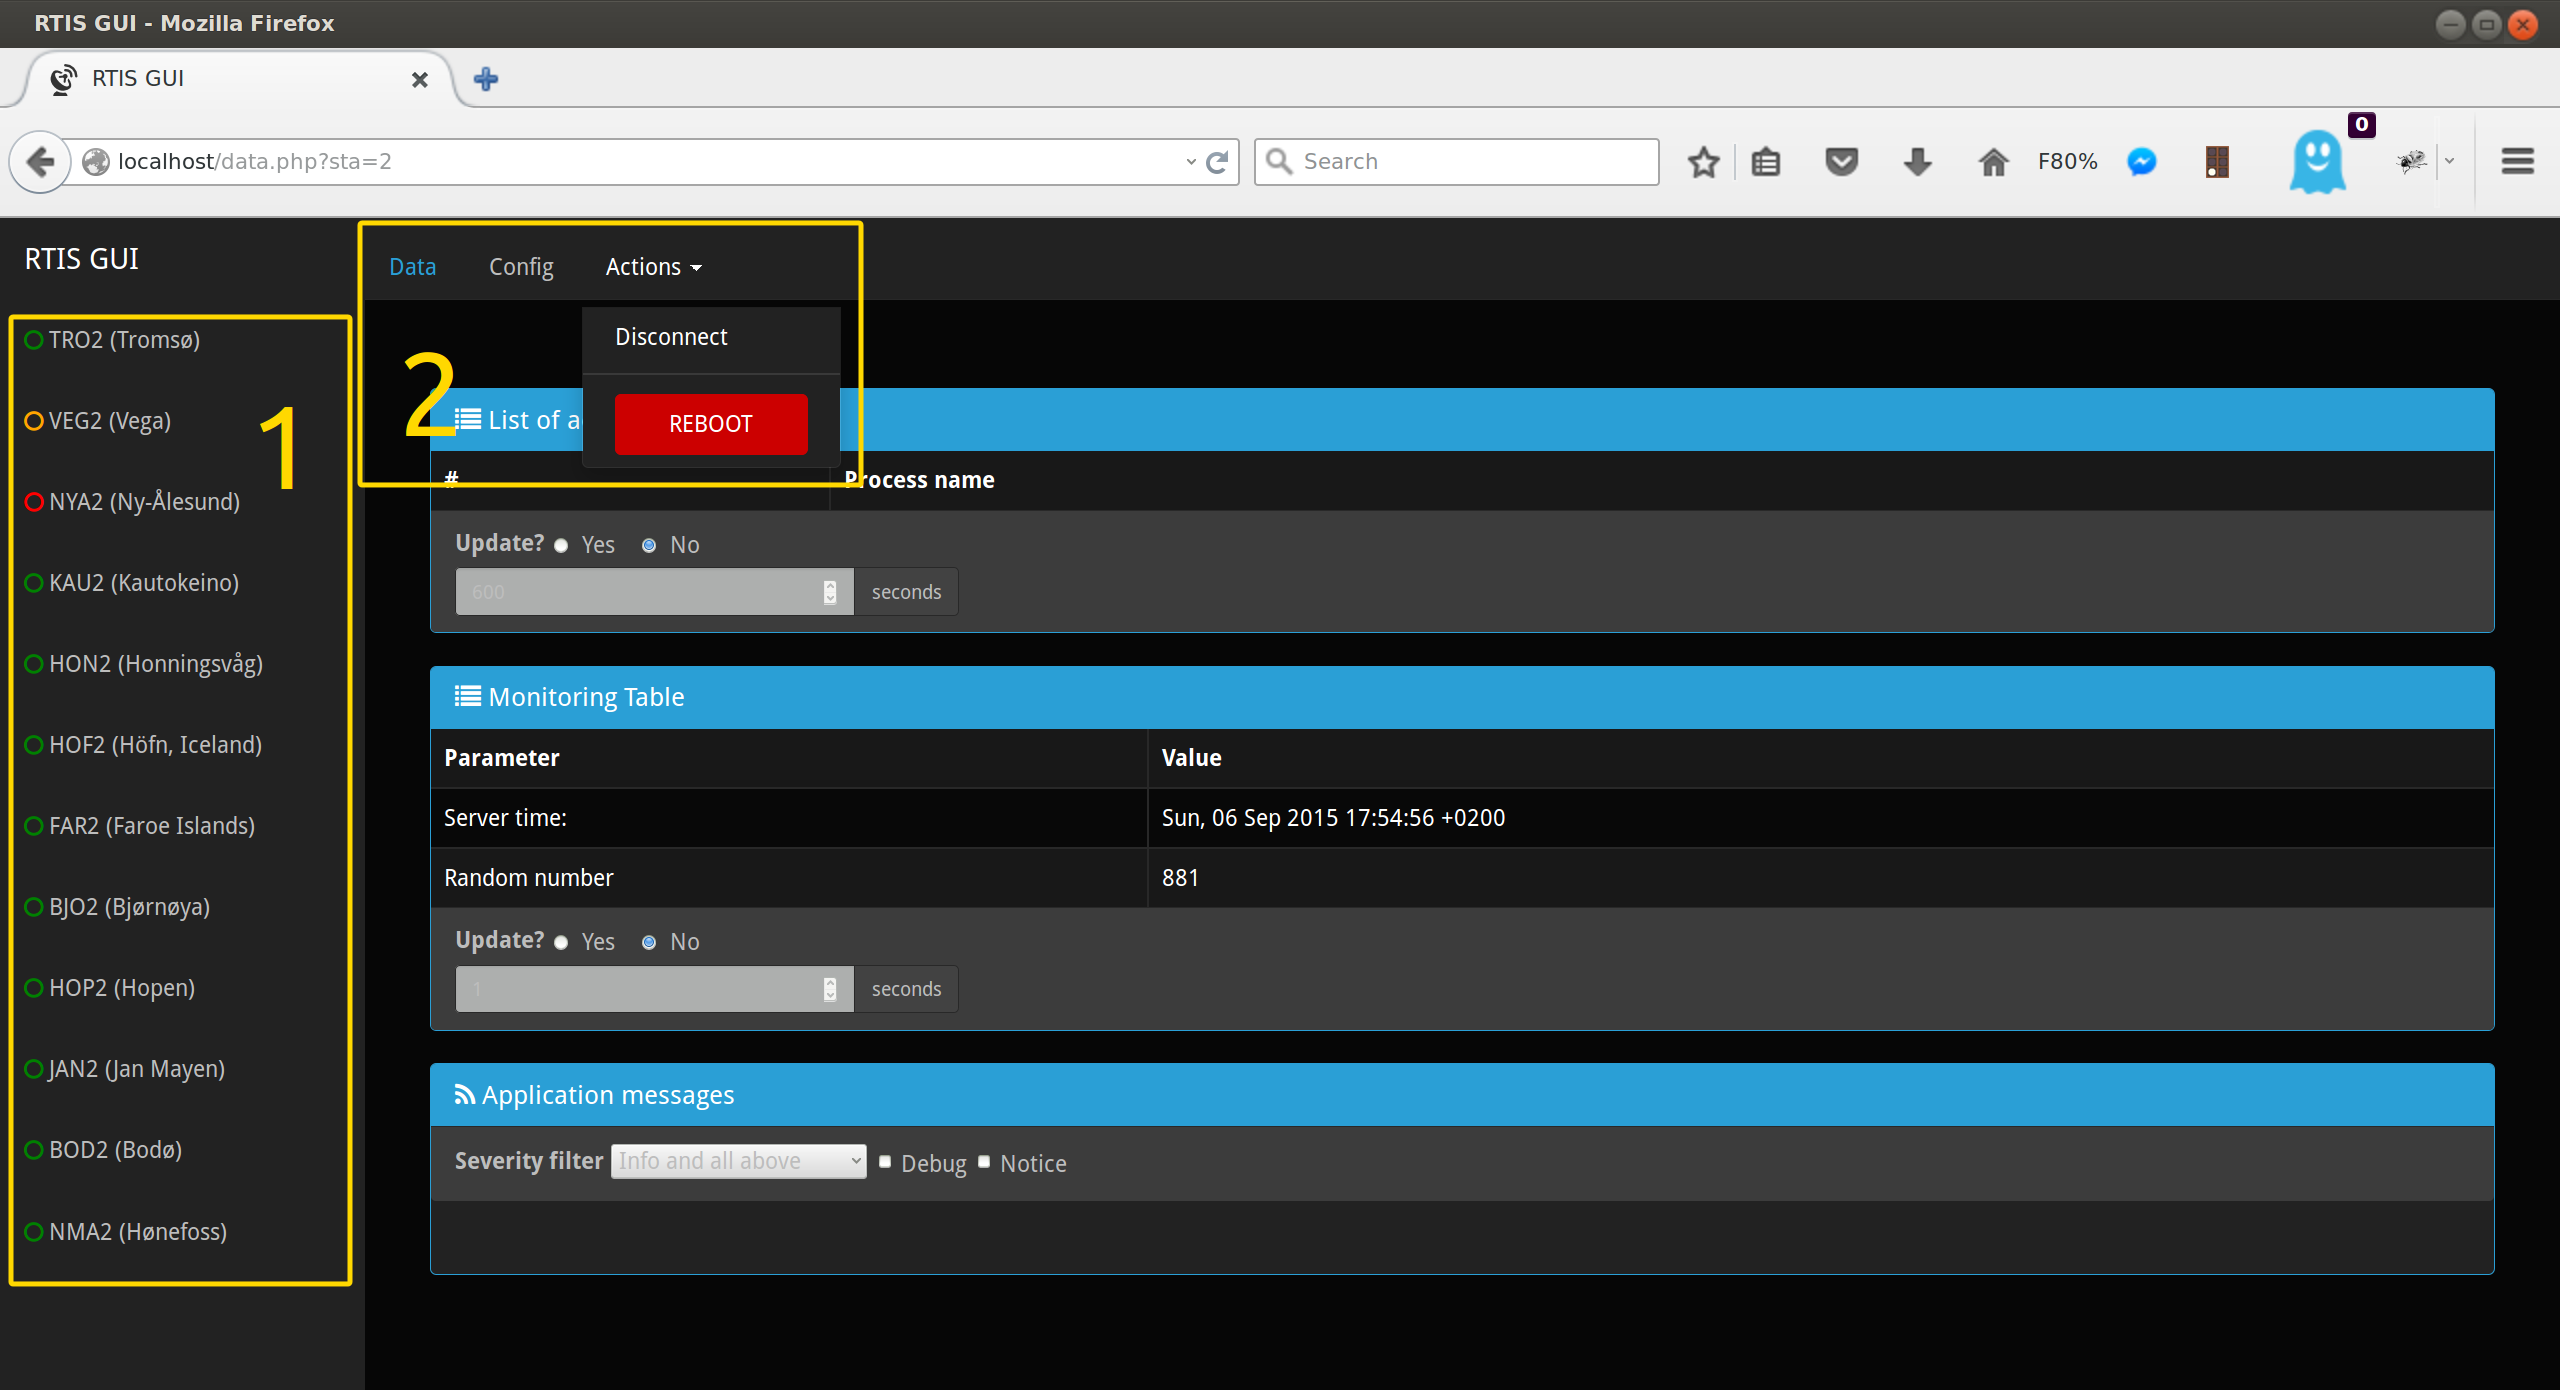
\includegraphics[width=1.1\textwidth]{Screenshot_Pinta}
	\caption{Screenshot of the interface, data tab}
\end{figure}

The two circled menus are present at all time when navigating the interface. The menu on the left, numbered 1, allows the user to choose the station he wants to monitor. It also indicate the state of every station thanks to the colour of the circles: green circles for healthy stations which send heartbeats with a "healthy" code, orange for non-healthy  stations whose heartbeats indicate failure, and red in case of a total absence of heartbeat.
The second menu, numbered 2, on top, is quite self-explanatory; once the user has chosen a station to connect to, it takes him to either the \textit{Data} page, to visualise monitoring data, or to the \textit{Config} page, for everything related to configuration files. The \textit{Disconnect} option on the \textit{Action} drop-down menu takes the user to the blank index page, and the \textit{Reboot} option leaves the user where he is, in order for him to see the data beginning to display again when the reboot of the remote station is complete.\\

For mobile devices, the menu 1 with the list of stations is minimised in the top right corner of the screen, and deploys on click.\\

\begin{figure}[ht]
	\centering
	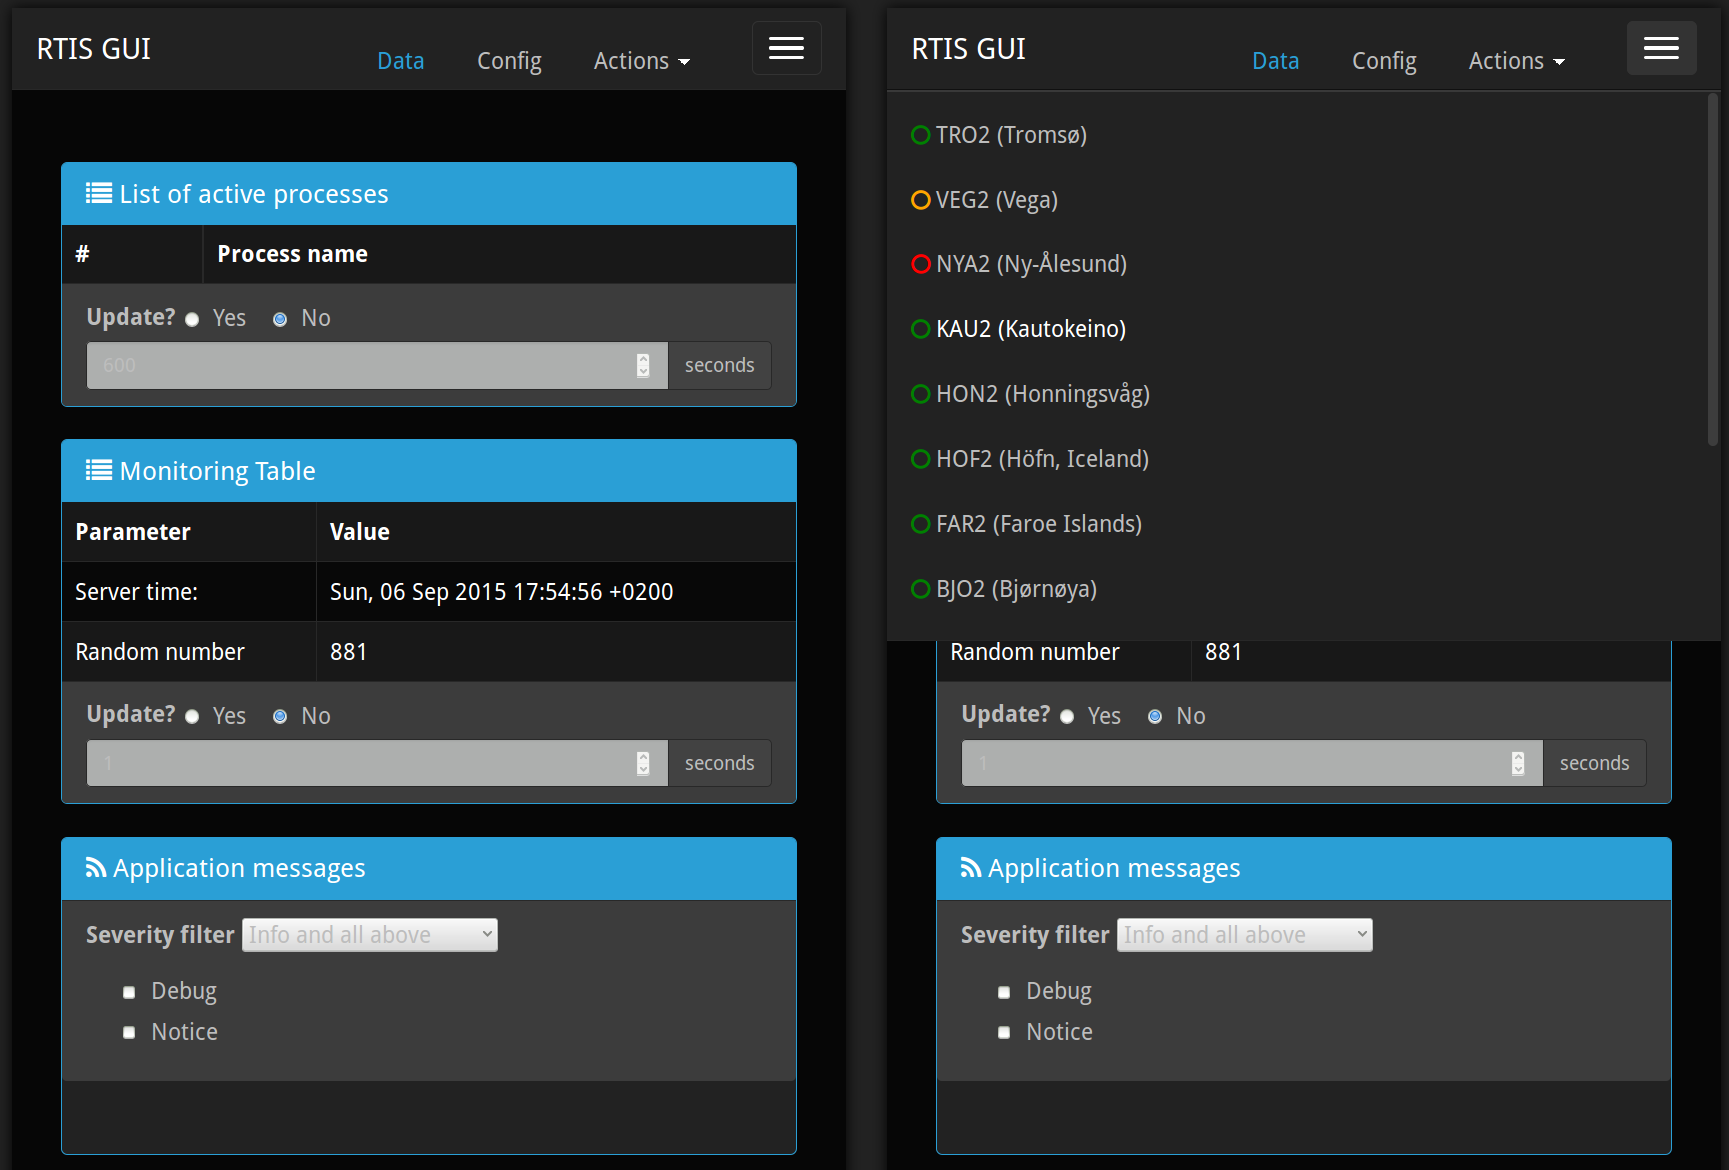
\includegraphics[width=\textwidth]{gui_mobile}
	\caption{Responsive design: minimised menu on the left, deployed menu on the right}
\end{figure}


\subsection{Receiving data}

When monitoring a station, the first thing to do is to make sure it is correctly functioning. The data tab is therefore the first tab the user is taken to when connecting to a station. This page can display the list of running RTIS processes (PROC), the monitoring table (MON) and/or the error messages from the RTIS software (ERR).\\
Each of this type of information has its own panel, and can be updated separately from the others. For MON and PROC, it is possible to choose whether to update or not, and if yes, at which frequency. The options to do so are located just under the display.
For ERR, it is possible to choose from a drop-down list a minimum severity level under which the messages will not be displayed. A "no message" option is also available. Since they are different than the regular options, the "Debug" and "Notice" filters have their own check-box, and can be chosen regardless of the "regular" severity filter.

In an effort to be as intuitive as possible, the choice of colours for the page has been made so that the different areas (title, information, settings) are easy to recognise. \\

When the data tab is first opened, the default options are that PROC would receive only one update and then be set to "no update". MON would be set to one update per second, and ERR would display all error messages except the special ones (Debug and Notice). The reason for not updating PROC by default is that it should not change. If everything is running like it should, there is no reason that a process would crash while we are monitoring the station. And if it is believed that it could happen, there is always the option to set the settings to "Update" manually.\\

The ERR panel will only display the ten most recent messages, and keeps the one thousand latest underneath. This amount can easily be changed in the code, but given the frequency of the messages, it has been agreed that it should be enough. Older messages are erased as new ones arrive. Each message is displayed with a colour and an icon depending on its severity. Please note that the example that follows has been done with dummy error messages composed of only random strings.\\

\begin{figure}[ht]
	\centering
	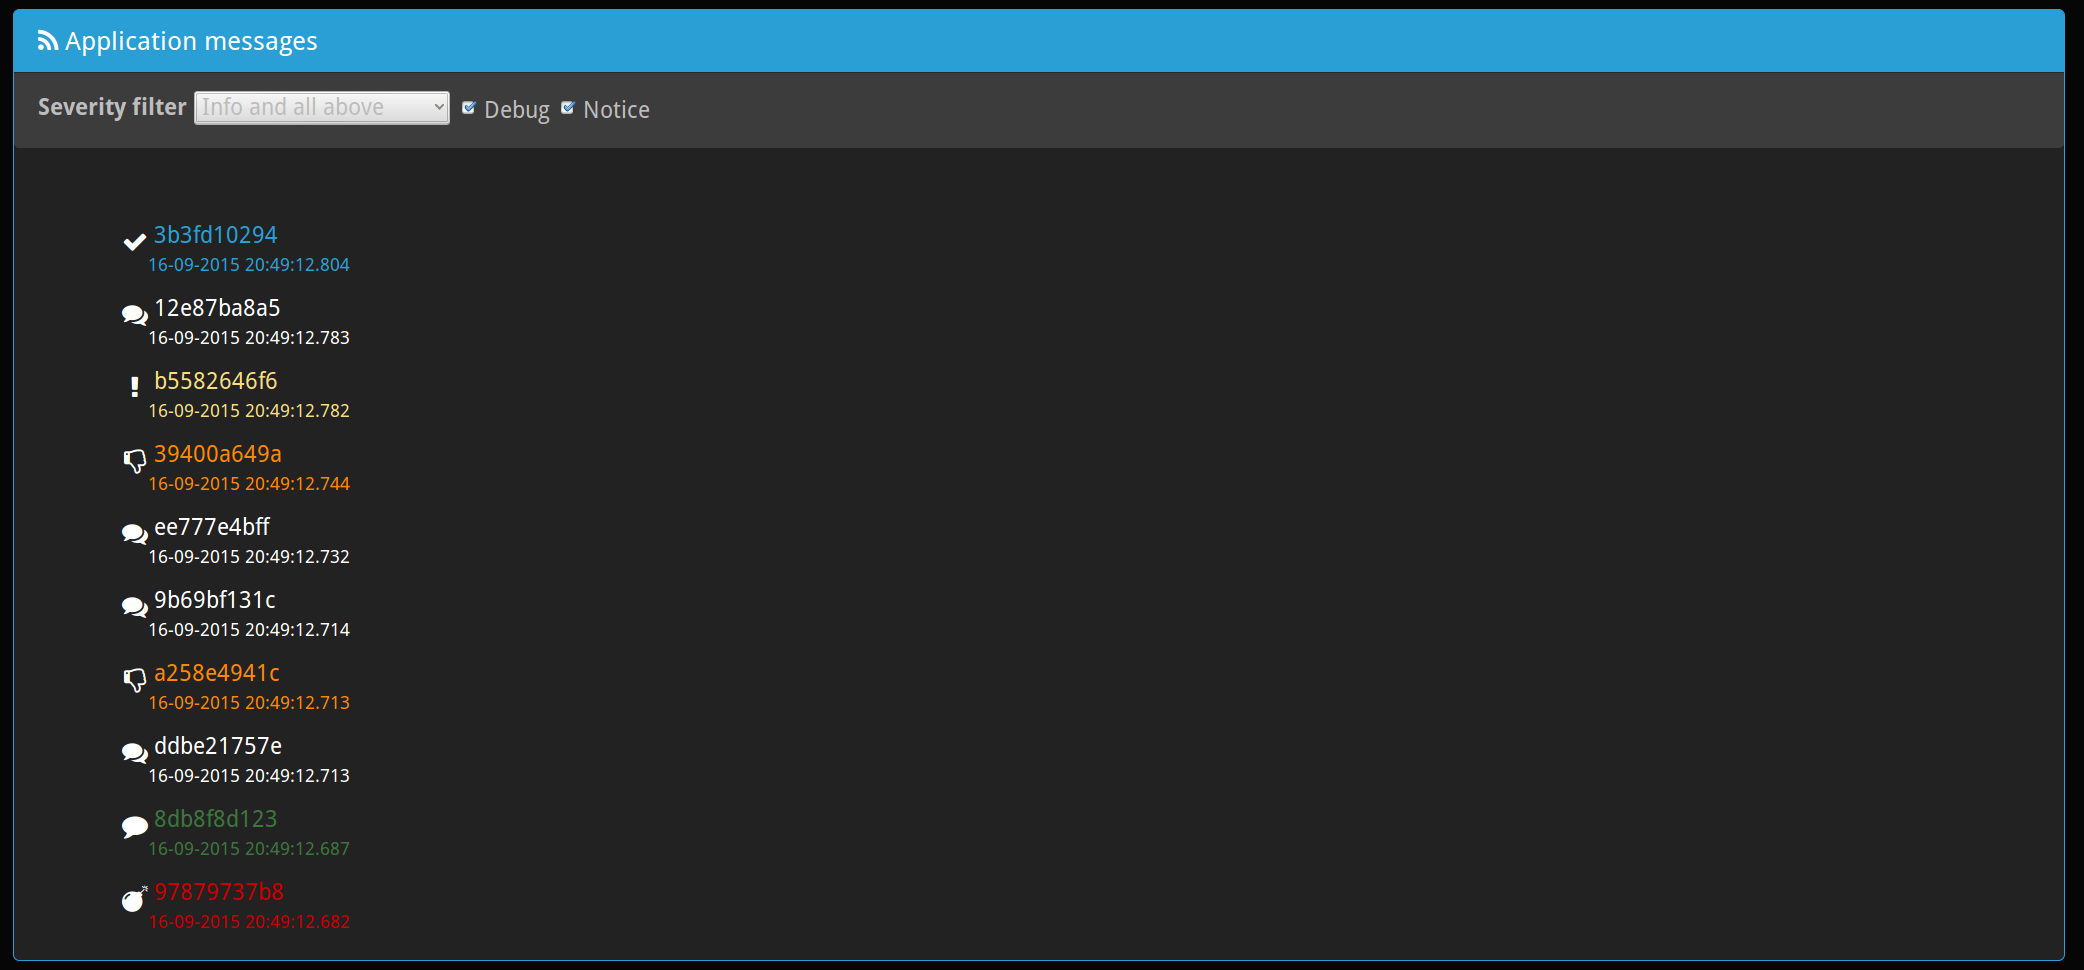
\includegraphics[width=\textwidth]{errPanel}
	\caption{The error messages panel}
\end{figure}

As we can see here, the messages are displayed in a way that their content is on top, with the time the error arose just underneath, in an attempt to be easily readable and understandable.\\

Each of these panels can be minimised by clicking on the blue title bar, and makes it possible to hide informations. It is for example possible to minimise the middle panel, so as to see both the top and the bottom one simultaneously, which would not be possible otherwise.\\

\begin{figure}[hb]
	\centering
	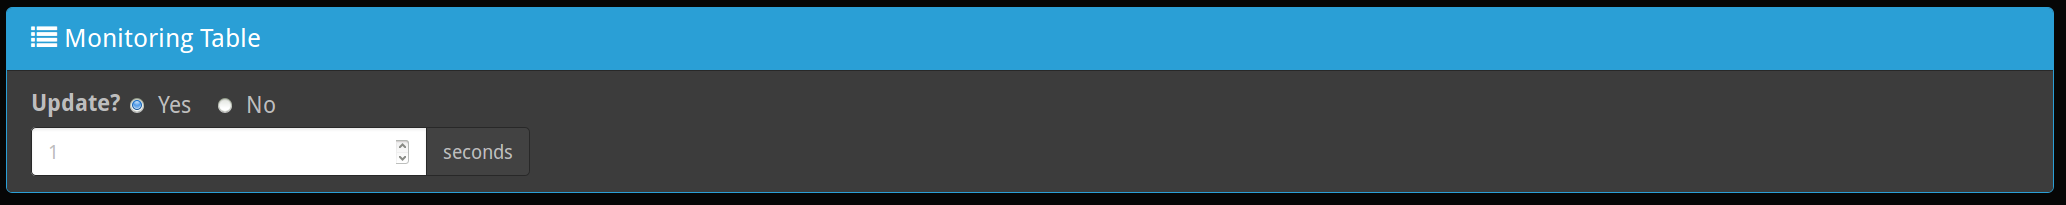
\includegraphics[width=\textwidth]{minimised}
	\caption{An example of a minimised panel}
\end{figure}


%-------------------------------------------------------------------------------
\newpage
\subsection{Sending \& saving configuration files}

\begin{figure}[ht]
	\centering
	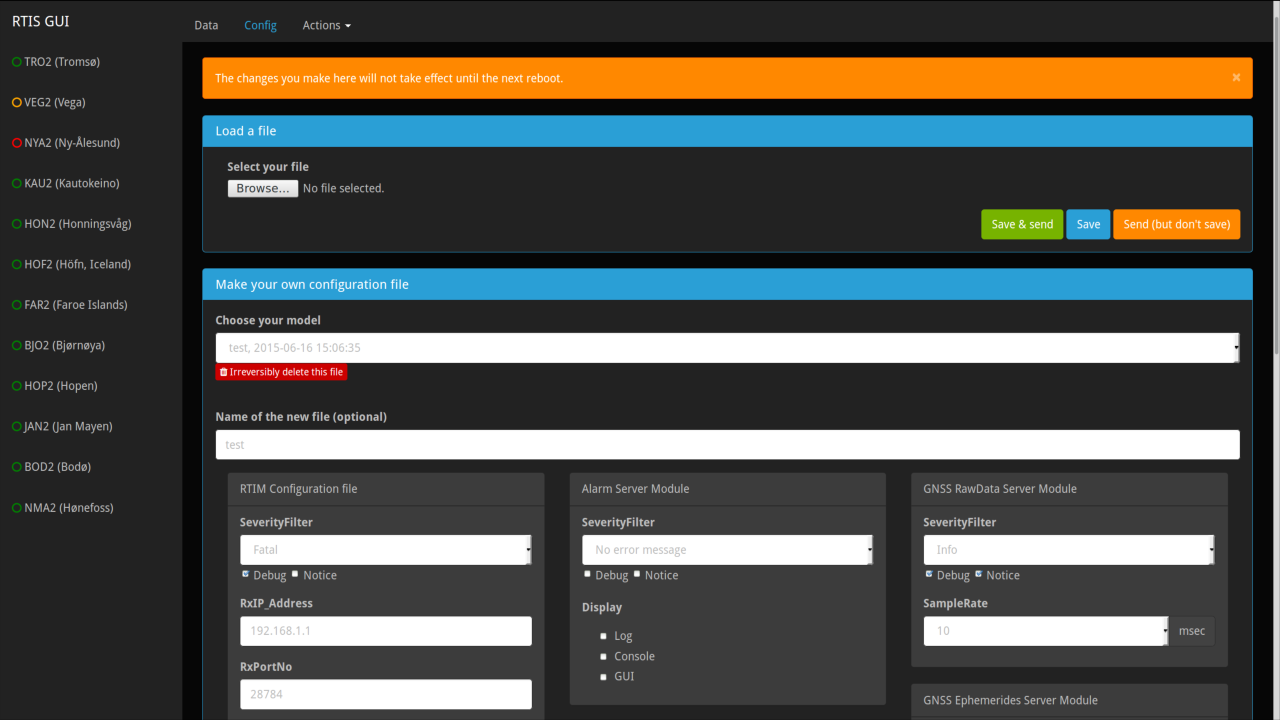
\includegraphics[width=\textwidth]{screenshotConfig}
	\caption{Screenshot of the config tab}
\end{figure}


The config tab is here to allow the user to send its own configuration files to the remote RTIS station. I chose to allow the file to be input either by a direct file upload or by a form that has to be manually completed, as either way can be practical depending on what the user wants to do. Going through the form can be longer than just uploading a file, but it allows to load an existing file and just modify a few fields. à, Moreover, the very idea of having to upload files from the device does not go well with the requirement of the web page being mobile-device friendly.\\

All the configuration files that are entered through this tool are stored into a database on the web server. This database only consists of one table, the configuration files, will not contain a lot of data, and is only ever asked to do simple read or write operations, without any join. I thus chose to use a basic mySQL relational database.\\

The idea is that whenever the user sends a configuration file to a station, this file has to be saved into the database, in order to be able to be reloaded later. When saving a file, it is possible to give it a name. While purely aesthetic, the name could make it easier to find it again later, instead of choosing a file based solely on its modification date.\\
To transfer data from the GUI to the database, the user has to choose between two options: \begin{itemize}
%\item sending the file to the station, and not saving the file in the database. This is not recommended, as the GUI will only display files from the database and thus will not know what file is active: we would have no idea of what is currently running on the remote station;
\item saving the configuration file in the database and sending the configuration file to the station;
\item just saving the file in the database without sending it, to continue working on it later.
\end{itemize}
These two options will call the “Save” function of the configuration file module. When saving a file in the database, a new field is added to it: the "active" attribute. It is used to know which file is the current file in the remote station.

The process of saving a file in the database is explained in a UML activity diagram, figure~\ref{fig:saveConfig}.\\

\begin{figure}[ht]
	\centering
	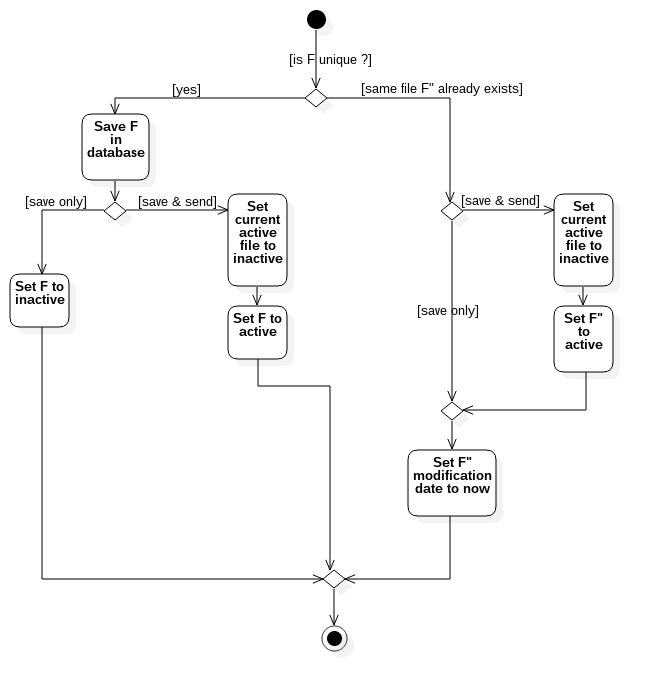
\includegraphics[width=\textwidth]{saveConfigInDb}
	\caption{Activity diagram of saving a file F in the database.}
	\label{fig:saveConfig}
\end{figure}

Before saving a configuration file however, be it by direct file input or through the use of the form, all of the values it contains are checked, for malicious input, first, but also to see if the values entered correspond to what is expected: is the port number an integer? Is it lower than 65536? If any of the values is incorrect, a message is printed on the interface explaining what the problem is.\\
When entering the configuration file through the form, the input fields are accepted or rejected as they are filled, with an explicit colour code, so that the user can see what is wrong in case of error, or have a confirmation that what he typed is acceptable. 

\begin{figure}[ht]
	\centering
	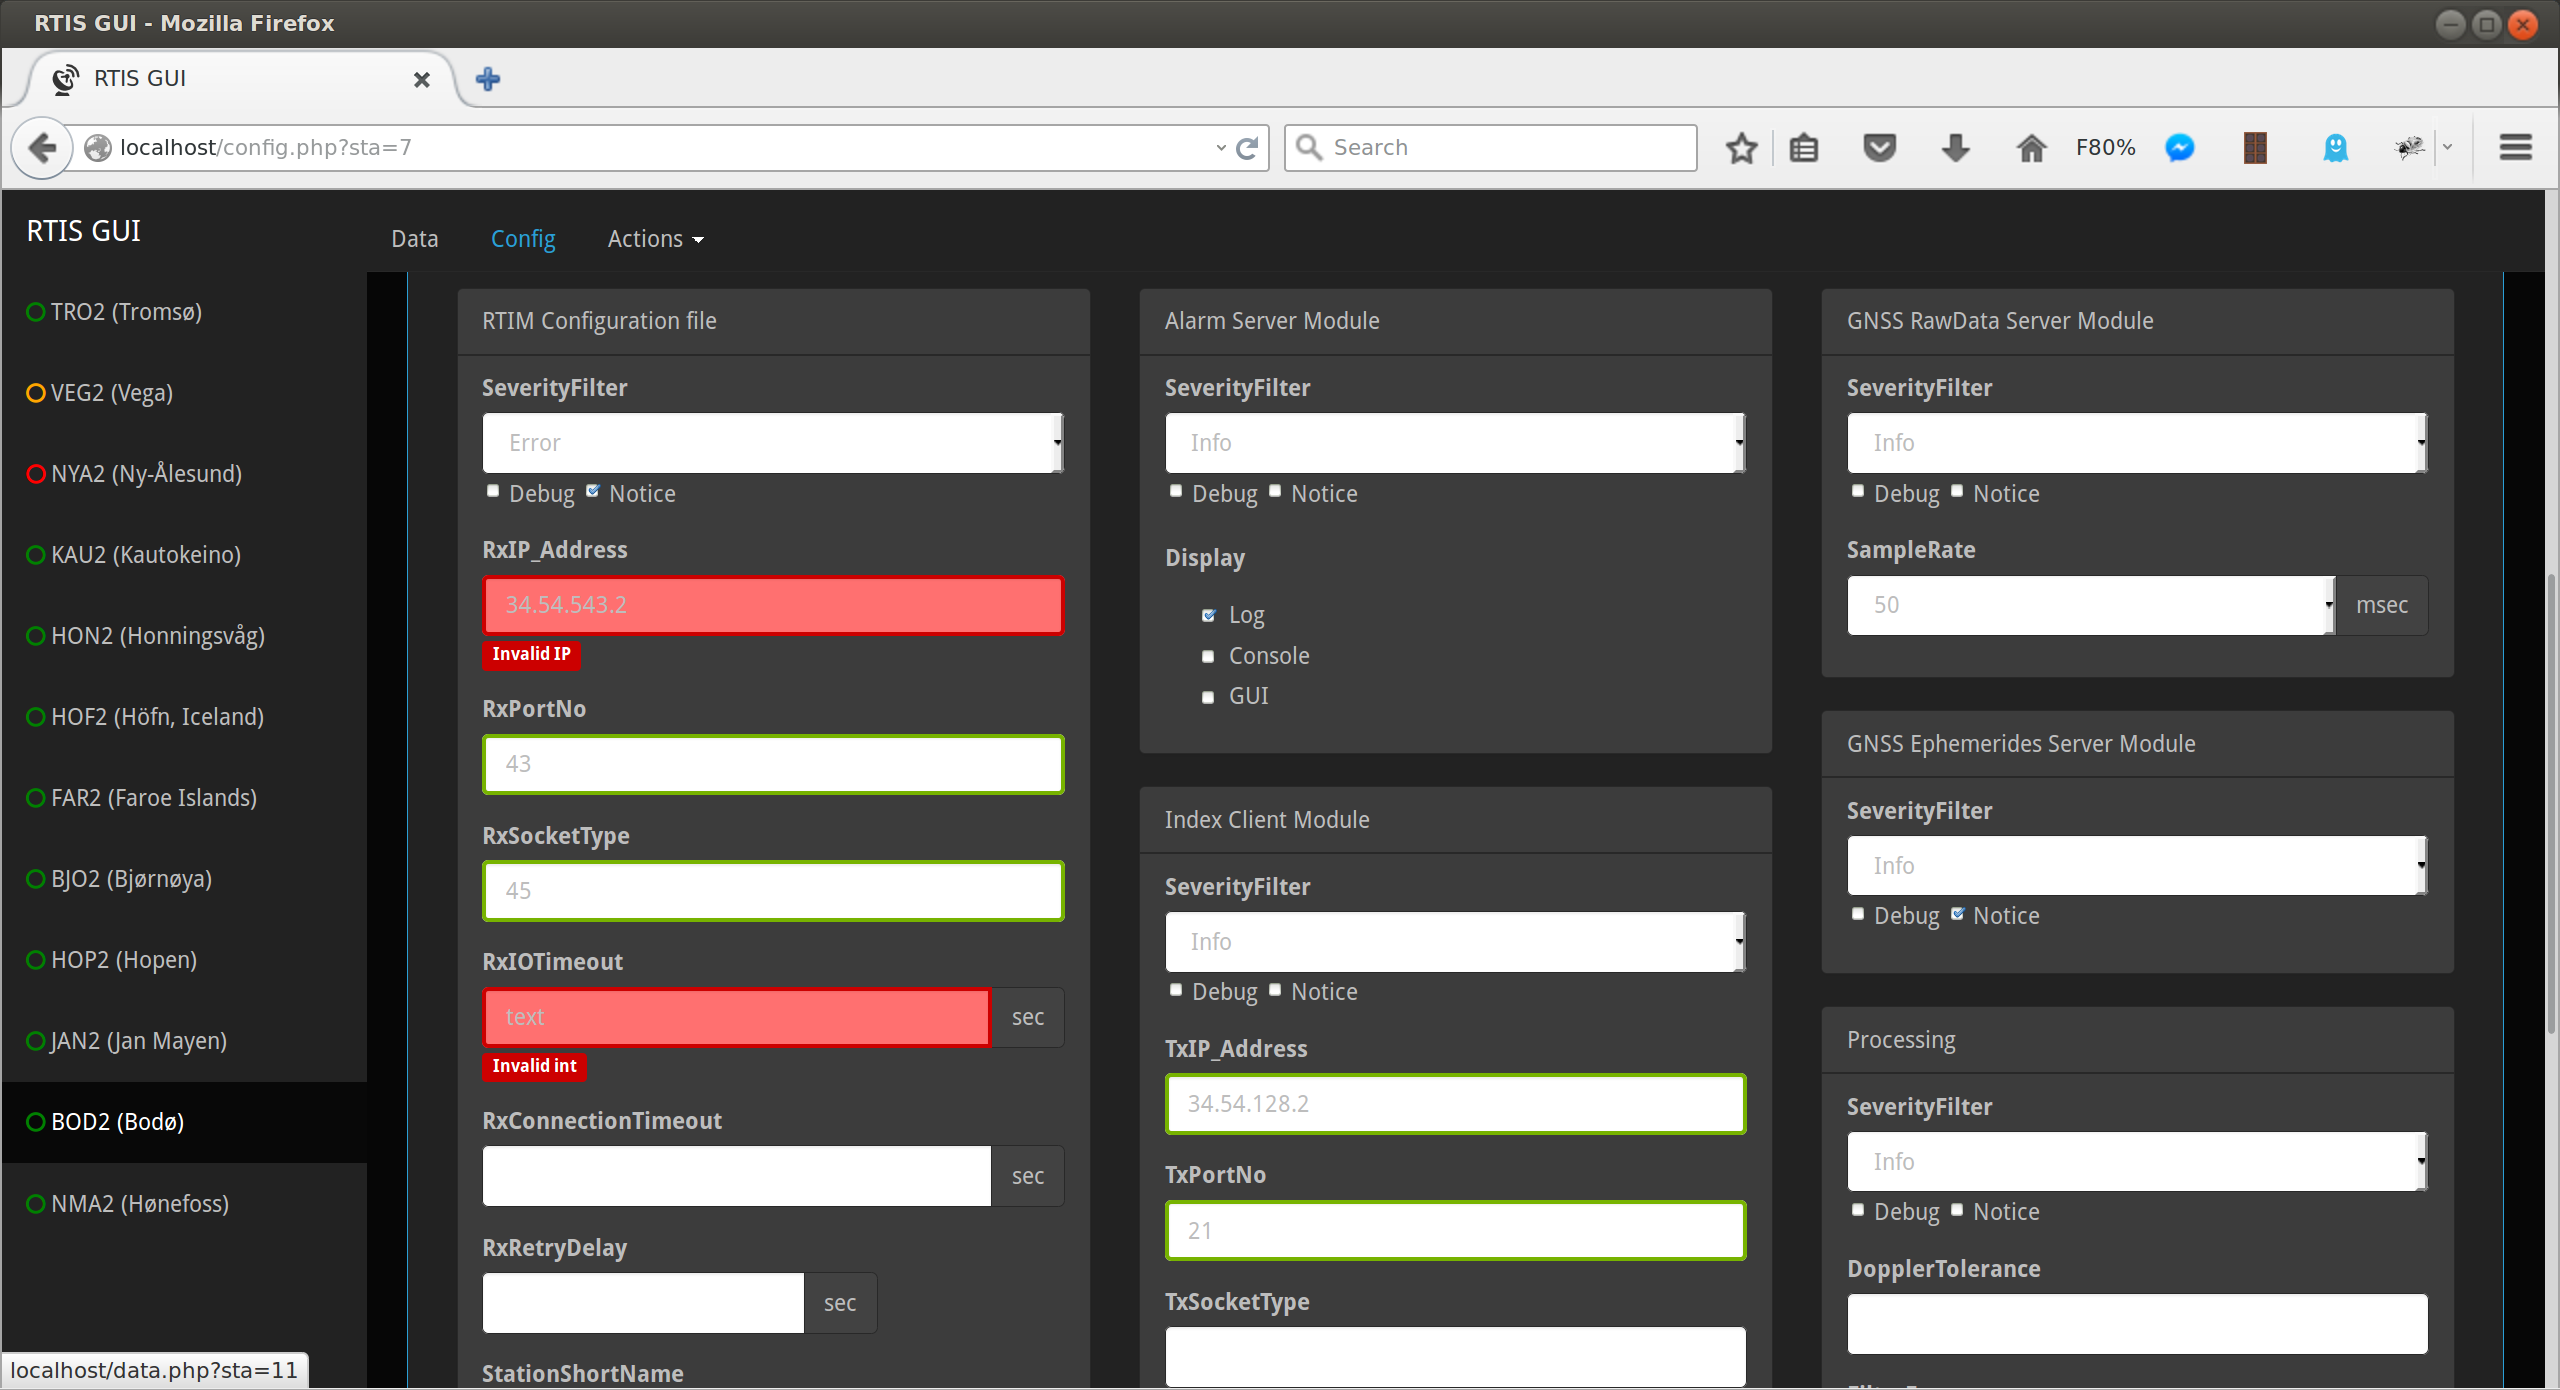
\includegraphics[width=\textwidth]{configFileValidation}
	\caption{Screenshot of filling in the form for a configuration file, halfway through: successfully filled input fields are circled in green, errors are filled in red with a little explanation text.}
\end{figure}

To get a list of files from the database, the GUI calls the function “Display a drop-down list” whenever the user goes to the configuration file modification page. This function queries to the database to get the list of names of the configuration files for the current station, and formats it so that it can directly be included in the HTML code as a drop-down list. Once the drop-down list is made, the user can choose one of its elements, that is to say one of the previous configuration files. Choosing an element triggers the “Prefill fields” function, which queries the database for all of the information concerning the selected configuration file, and prefills the GUI fields accordingly. Initially, the fields are filled with the values from the current active configuration file on the RTIS installation, which is the only “active” file in the database for the current station. If no active file is found, then the latest modified station is taken. Finally, if the station is new and has no configuration file in the database at all, the fields are left blank.\\
It is also possible to remove a file from the database from the GUI by selecting it in the drop-down list and clicking on the “Delete” button. This calls the “Delete” function. The active file cannot be deleted.

%-------------------------------------------------------------------------------
\newevenpage
\chapter*{Conclusion}
  \addcontentsline{toc}{part}{Conclusion}
  \vspace{1.5cm}

\newevenpage
\begin{appendices}
\label{beginappendices}

\annexe{Process Table \& Monitor Data Structures}
\label{structures}

\begin{lstlisting}[language=C]
/*
*******************************************************************************
RTIS Process Table
*******************************************************************************
*/
typedef struct
{
	pid_t 			Pid;
	char	 	    		IntName[GL_PROCESS_NAME_SIZE];
	INT32			iStartTime;
	INT8 			ActionFlag;
}rtis_TProcessTableInfo;

/*
*******************************************************************************
RTIS Monitor Table
*******************************************************************************
*/
typedef struct
{
	UINT32			uiCurWeek;
	UINT32			uiCurTow;
	INT32			iCurDataTbl;
	INT32			iReadyDatasetCount;
	INT32			iCurIndex;
	INT32			iNoOfRawMeas;
	INT32			iNoOfIQMeas;
	INT32			iNoOfLostRawMeas;
	INT32			iNoOfLostIQMeas;
	INT32			iOther;
	INT32			iTotNoOfRawMeas;
	INT32			iTotNoOfIQMeas;
	INT32			iTotOther;
}rtis_TMonitorInfo;


\end{lstlisting}

\annexe{Example of a RTIS configuration file}
\label{configfile}

\lstinputlisting[language=Lisp]{resources/rtis_config.cfg}

\annexe{Statement of Work}
\label{SOW}

\includepdf[pages={1,2,3,4,5,6,7,8,9,10}]{resources/statementOfWork.pdf}

\annexe{SATREF Extended Message Protocol Specification}
\label{satref}
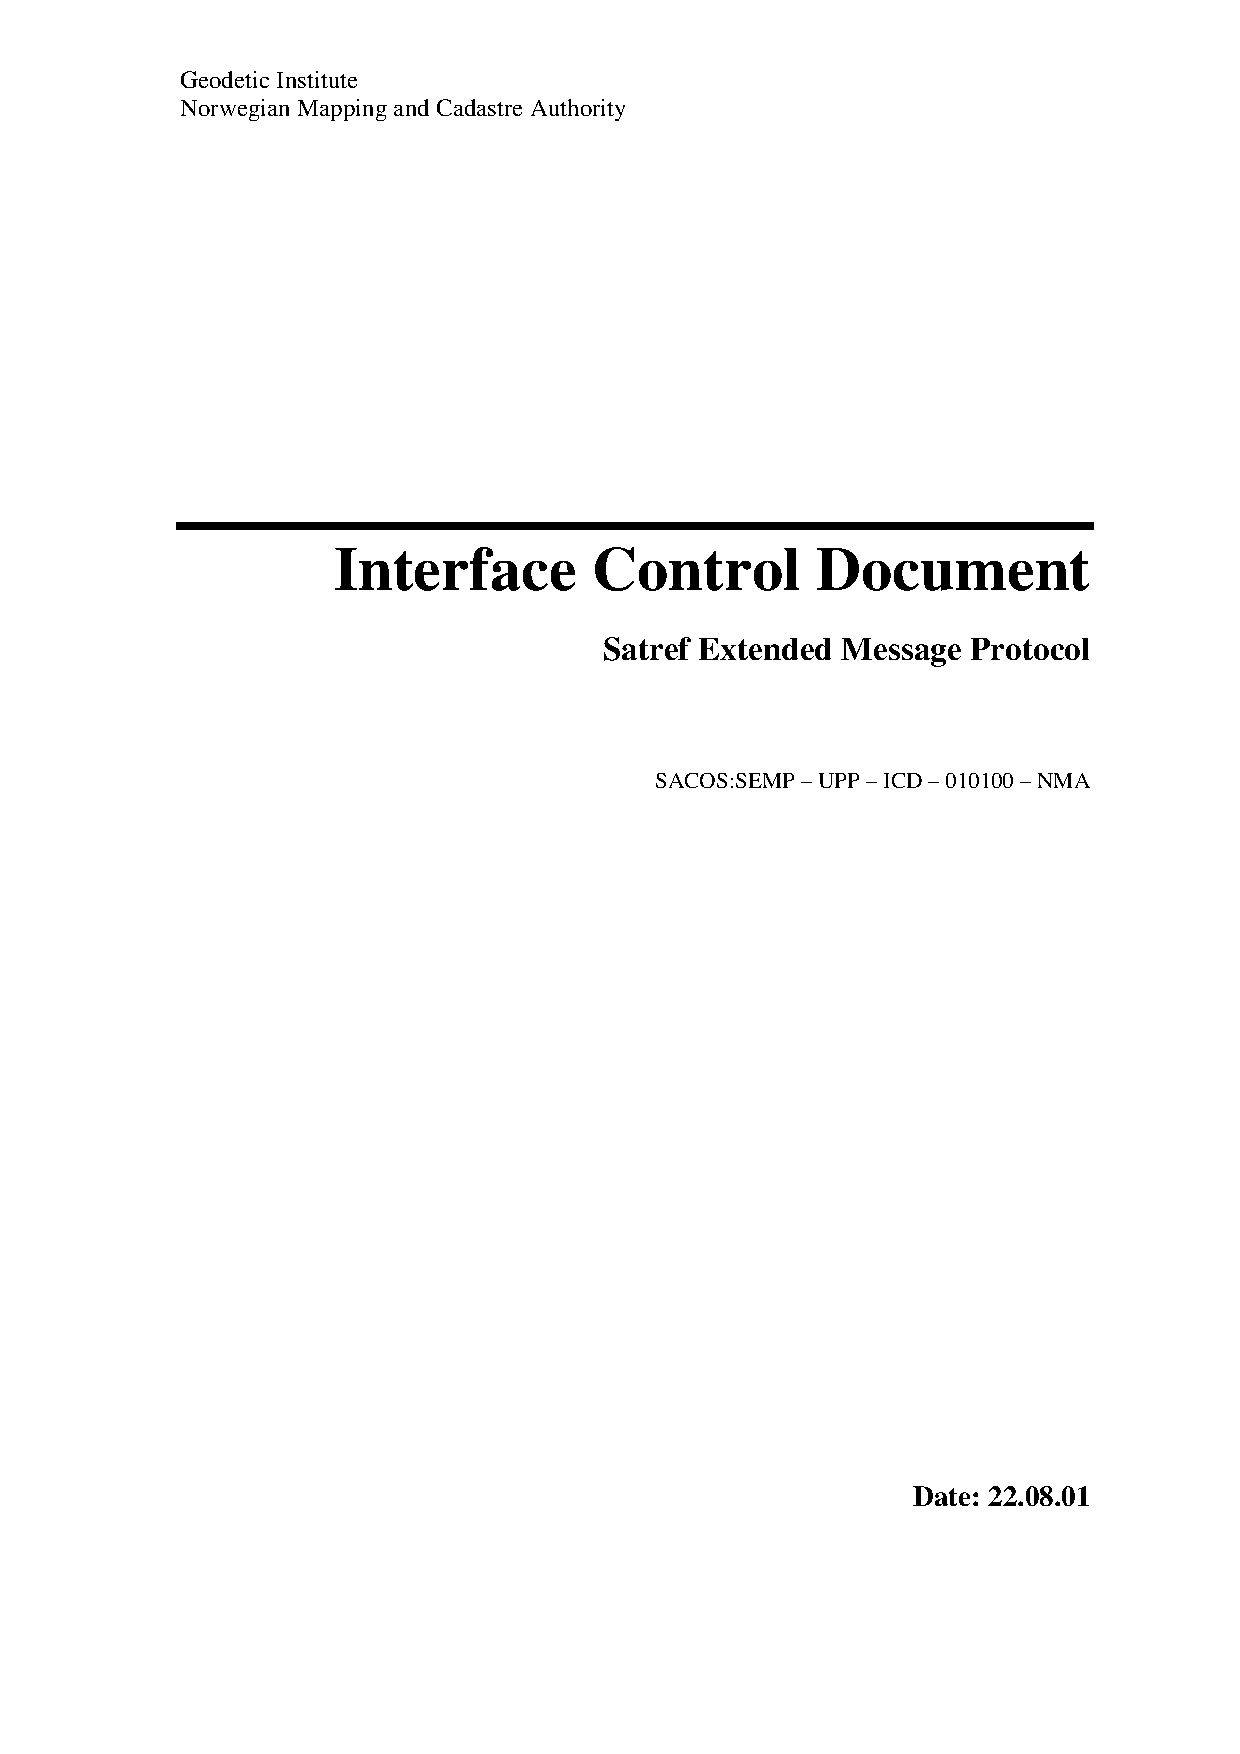
\includepdf[pages={-}]{resources/SATREF.pdf}


\end{appendices}


\end{document}